\documentclass[10pt,a4paper]{article}

% ---------------------------------------------------------------------------
% From zero to the phi^4 laboratory: a self-contained primer.
% Build: cd reports && tectonic -X compile theory-primer-2026-10-01.tex
% Figures: python tools/make_primer_figs.py (primer-*.pdf); the closing chapter
% also uses fig-field-potential.pdf and fig-field-sweep.pdf (tools/make_field_*.py).
% Parts live in reports/primer/.
% ---------------------------------------------------------------------------

\usepackage[T1]{fontenc}
\usepackage[utf8]{inputenc}
\usepackage{lmodern}
\usepackage[margin=2.1cm,top=2.0cm,bottom=2.2cm]{geometry}
\usepackage{microtype}
\usepackage{amsmath,amssymb,amsthm}
\usepackage{booktabs}
\usepackage{enumitem}
\usepackage{graphicx}
\usepackage{xcolor}
\usepackage[most]{tcolorbox}
\usepackage{tikz}
\usetikzlibrary{positioning,arrows.meta}
\usepackage{titlesec}
\usepackage[hidelinks]{hyperref}

\graphicspath{{figures/}}
\setlength{\parskip}{0.3em}
\setlength{\parindent}{0pt}
\titleformat{\section}{\Large\bfseries}{\thesection}{0.6em}{}
\titlespacing*{\section}{0pt}{1.2em}{0.5em}
\titleformat{\subsection}{\normalsize\bfseries}{\thesubsection}{0.5em}{}
\titlespacing*{\subsection}{0pt}{0.9em}{0.3em}
\setlist{itemsep=0.15em,topsep=0.25em}

\theoremstyle{plain}
\newtheorem{proposition}{Proposition}[section]
\newtheorem{lemma}[proposition]{Lemma}
\newtheorem{corollary}[proposition]{Corollary}
\theoremstyle{definition}
\newtheorem{definition}[proposition]{Definition}
\newtheorem{example}[proposition]{Example}

\definecolor{keyc}{HTML}{1c5cab}
\definecolor{projc}{HTML}{1a8a62}
\definecolor{warnc}{HTML}{c24d1f}
\newtcolorbox{keyidea}{enhanced,breakable,colback=keyc!4,colframe=keyc,boxrule=0.5pt,arc=1.5pt,
  left=5pt,right=5pt,top=3pt,bottom=3pt,fonttitle=\bfseries\small,title=Key idea}
\newtcolorbox{inproject}{enhanced,breakable,colback=projc!4,colframe=projc,boxrule=0.5pt,arc=1.5pt,
  left=5pt,right=5pt,top=3pt,bottom=3pt,fonttitle=\bfseries\small,title=In our project}
\newtcolorbox{caution}{enhanced,breakable,colback=warnc!4,colframe=warnc,boxrule=0.5pt,arc=1.5pt,
  left=5pt,right=5pt,top=3pt,bottom=3pt,fonttitle=\bfseries\small,title=Careful}

\newcommand{\E}{\mathbb{E}}
\newcommand{\R}{\mathbb{R}}
\newcommand{\Var}{\operatorname{Var}}
\newcommand{\Cov}{\operatorname{Cov}}
\newcommand{\N}{\mathcal{N}}
\newcommand{\KL}{\mathrm{KL}}
\newcommand{\dd}{\,\mathrm{d}}
\newcommand{\Th}{\Theta}
\newcommand{\En}{\mathcal{E}}
\newcommand{\Zp}{\mathcal{Z}}
\newcommand{\fwd}{\overrightarrow{m}}
\newcommand{\bwd}{\overleftarrow{m}}
\newcommand{\code}[1]{\texttt{\small #1}}
\newcommand{\T}{^{\top}}

\begin{document}

\begin{titlepage}
\vspace*{3cm}
{\Huge\bfseries From Zero to the $\phi^4$ Laboratory\par}
\vspace{0.6cm}
{\Large A self-contained primer on the mathematics behind structured denoising\par}
\vspace{1.2cm}
{\large Kalman filtering and smoothing \textperiodcentered{} Fourier and Hermite analysis \textperiodcentered{}
EM and its generalisations \textperiodcentered{} Fisher information and quasi-likelihood \textperiodcentered{}
hidden Markov models, Markov random fields and belief propagation \textperiodcentered{}
the Allen--Cahn equation and its stochastic version \textperiodcentered{} and how they meet\par}
\vfill
{\normalsize Prepared for Giovanni Mantovani \textperiodcentered{} 1 October 2026\\[0.2em]
repository \code{markov-score-diffusion-icml}\\ branch \code{claude/phi4-field-2026-10-01}\par}
\vspace{0.4cm}
{\small Every figure is generated from the project's own code (\code{tools/make\_primer\_figs.py});
every number quoted from an experiment names the experiment and says whether it is frozen or a preview.\par}
\end{titlepage}

\section*{How to read this primer}

The project asks one question: given many noisy copies of sequences that come from a
one-dimensional physical system, can we learn the system's local rule and then compute the
\emph{exact} best denoiser? Answering it uses ten pieces of mathematics that are usually
taught in ten different courses. This primer builds each of them from the ground up, in an
order where every chapter only uses what came before.

\begin{itemize}
\item \textbf{Part I, foundations} (\S1--3). The calculus, linear algebra and probability you need,
  including the one trick used everywhere (completing the square), conditional expectation as the
  best predictor, and Markov chains.
\item \textbf{Part II, inference on chains} (\S4--6). Noise, scores and Tweedie's formula; the Kalman
  filter and smoother; hidden Markov models, Markov random fields and belief propagation.
\item \textbf{Part III, spectral tools} (\S7--8). Fourier analysis (why noise erases fine detail) and
  Hermite polynomials (why fourth-order structure fades like $e^{-4t}$).
\item \textbf{Part IV, learning} (\S9--10). Maximum likelihood, the EM algorithm and its general forms;
  Fisher information, the Cram\'er--Rao bound, quasi-likelihood.
\item \textbf{Part V, physics} (\S11--12). From a ball rolling in a valley to the Allen--Cahn equation
  and its stochastic version; the transfer operator that turns a field into a Markov chain.
\item \textbf{Part VI, the new theory} (\S13). The tilted walk, reversibility, the learned pair energy,
  and what the experiments have measured.
\end{itemize}

Three kinds of boxes recur. \emph{Key idea} boxes state the one thing to remember. \emph{In our
project} boxes say where the idea lives in the code and experiments. \emph{Careful} boxes flag the
traps that have cost us time. Proofs are given whenever they are short enough to be read in a
minute; the longer ones are sketched with the step that matters.

\tableofcontents
\clearpage

% Part I: foundations (sections 1-3)
\addcontentsline{toc}{part}{Part I \quad Foundations}
\section{The toolbox}\label{sec:toolbox}

\subsection{Slopes, curvature, and the second difference}

A function $f$ assigns a number $f(x)$ to every number $x$. Its \emph{derivative} $f'(x)$ is the slope of
the graph at $x$: for a small step $h$,
\[
  f'(x)\approx\frac{f(x+h)-f(x)}{h}.
\]
The second derivative $f''(x)$ is the slope of the slope, which measures curvature: positive where the graph
bends upwards like a cup, negative where it bends down like a cap. Taylor's formula says that near $x$ every
smooth function looks like a parabola,
\begin{equation}\label{eq:taylor}
  f(x+h)=f(x)+h\,f'(x)+\tfrac{1}{2}h^2f''(x)+\tfrac16h^3f'''(x)+\dots
\end{equation}

Write \eqref{eq:taylor} once with $+h$ and once with $-h$ and add. The odd powers cancel, and
\begin{equation}\label{eq:seconddiff}
  \frac{f(x+h)-2f(x)+f(x-h)}{h^2}=f''(x)+O(h^2).
\end{equation}
The left side is the \emph{second difference}. Rewrite it as $\frac{2}{h^2}\big[\tfrac12(f(x+h)+f(x-h))-f(x)\big]$:
it is the gap between the average of the two neighbours and the value at the point. It is positive when the
point sits below its neighbours, negative when it sits above.

\begin{keyidea}
The second difference \eqref{eq:seconddiff} is all a \emph{Laplacian} is in one dimension. When physicists
write $\partial_x^2\phi$ or $\nabla^2\phi$ for a quantity $\phi$ that varies along a line, they mean ``how far
$\phi$ at a point is below the average of its neighbours'', in the limit of close neighbours. In more
dimensions one adds the same quantity for each direction. We will meet it as the force of the springs that
hold a string together (\S\ref{sec:allencahn}).
\end{keyidea}

A function of several variables $f(x_1,\dots,x_n)$ has \emph{partial derivatives} $\partial f/\partial x_i$:
the slope in direction $i$ with the others held fixed. Collected in a vector they form the \emph{gradient}
$\nabla f$, which points in the direction in which $f$ increases fastest.

\subsection{Integrals as sums, and the grid}

The integral $\int_a^b f(x)\dd x$ is the area under the graph. Chop $[a,b]$ into $N_g-1$ intervals of width
$\delta$ with points $u_1,\dots,u_{N_g}$; then
\begin{equation}\label{eq:trapezoid}
  \int_a^b f(x)\dd x\approx\sum_{k=1}^{N_g}w_k\,f(u_k),\qquad w_k=\delta\ \text{except}\ w_1=w_{N_g}=\delta/2 .
\end{equation}
This is the \emph{trapezoid rule}; its error shrinks like $\delta^2$. Every integral in this project is done
this way: on $N_g=401$ points spread over $[-8,8]$, so $\delta=0.04$.

\subsection{Exponentials, logarithms, and why we compute in logs}

The exponential turns sums into products, $e^{a+b}=e^ae^b$, and the logarithm turns products back into sums.
Probabilities of long sequences are products of many numbers smaller than one, which underflow a computer
(in double precision $e^{-800}$ is exactly zero). So we store logarithms, and to add numbers stored as logs
we use the \emph{log-sum-exp} identity
\[
  \log\sum_k e^{y_k}=m+\log\sum_k e^{y_k-m},\qquad m=\max_k y_k,
\]
which never overflows because every exponent on the right is at most zero.

\subsection{Vectors, matrices, eigenvectors}

A vector is a list of numbers, a matrix a table. The product of two matrices is
\begin{equation}\label{eq:matprod}
  (AB)_{kj}=\sum_m A_{km}B_{mj},
\end{equation}
a sum over an intermediate index $m$. Remember this shape: ``sum over the state in the middle'' is the one
operation that belief propagation repeats (\S\ref{sec:bp}). The transpose $A\T$ swaps rows and columns; $A$ is
\emph{symmetric} if $A=A\T$. The inverse $A^{-1}$ undoes $A$.

An \emph{eigenvector} $v$ of a square matrix $A$ is a direction that $A$ only stretches: $Av=\lambda v$, with
\emph{eigenvalue} $\lambda$. Two facts carry most of the weight in this primer.
\begin{itemize}
\item A symmetric matrix has real eigenvalues $\lambda_0\ge\lambda_1\ge\dots$ and eigenvectors $v_0,v_1,\dots$ that
  are mutually perpendicular and of unit length. It can be rebuilt from them, $A=\sum_n\lambda_nv_nv_n\T$, and so
  $A^N=\sum_n\lambda_n^Nv_nv_n\T$. For large $N$ the largest $|\lambda_n|$ dominates: \emph{repeated multiplication
  forgets everything except the leading eigenvector}. That is the power method, and it is the reason a long
  chain ``forgets'' its start.
\item \emph{Perron--Frobenius}: if every entry of $A$ is positive, the largest eigenvalue $\lambda_0$ is positive
  and unrepeated, and its eigenvector can be chosen with every entry positive.
\end{itemize}
A symmetric $A$ is \emph{positive definite} if $v\T Av>0$ for every nonzero $v$, equivalently if all its
eigenvalues are positive. Covariance matrices are of this kind.

\subsection{The Gaussian integral and completing the square}

The single most useful integral is
\begin{equation}\label{eq:gaussint}
  \int_{-\infty}^{\infty}e^{-x^2/2}\dd x=\sqrt{2\pi}.
\end{equation}
(Square it, read the square as an integral over the plane, and switch to polar coordinates; the angular
integral gives $2\pi$ and the radial one gives $1$.) The single most useful trick is \emph{completing the
square}:
\begin{equation}\label{eq:complete}
  -\tfrac{A}{2}x^2+Bx=-\tfrac{A}{2}\Big(x-\tfrac{B}{A}\Big)^2+\tfrac{B^2}{2A}\qquad(A>0).
\end{equation}
It says that any exponent that is quadratic in $x$ describes a bell curve centred at $B/A$ with width
$1/\sqrt A$. Products of Gaussian bumps are Gaussian bumps because their exponents add, and the sum of two
quadratics is a quadratic. The whole of the Kalman filter is this sentence applied repeatedly.

\paragraph{Check yourself.}
\begin{enumerate}[label=\thesection.\arabic*,leftmargin=2.2em]
\item Show that the second difference of $f(x)=x^3$ equals $6x$ exactly, for every $h$. Why is there no error term?
\item The matrix $A=\begin{pmatrix}2&1\\1&2\end{pmatrix}$ has positive entries. Find its eigenvalues and eigenvectors, and say in which
  direction $A^Nv$ points for large $N$, whatever the starting vector $v$ (unless $v$ is special).
\end{enumerate}

\section{Probability from scratch}\label{sec:prob}

\subsection{Random variables, densities, expectations}

A random quantity $a$ is described by its \emph{density} $p(a)$: the probability that $a$ lands in a tiny
interval $[u,u+\dd u]$ is $p(u)\dd u$, and $\int p=1$. The \emph{expectation} of any function of $a$ is the
weighted average
\[
  \E[f(a)]=\int f(u)\,p(u)\dd u .
\]
The mean is $\mu=\E[a]$, the variance $\Var(a)=\E[(a-\mu)^2]$, the standard deviation its square root. For two
quantities the covariance $\Cov(a,b)=\E[(a-\E a)(b-\E b)]$ measures whether they move together, and the
correlation divides it by both standard deviations, landing in $[-1,1]$.

Two random quantities have a \emph{joint} density $p(a,b)$. Integrating one away gives the \emph{marginal},
$p(a)=\int p(a,b)\dd b$. Fixing one gives the \emph{conditional},
\[
  p(a\mid b)=\frac{p(a,b)}{p(b)},
\]
the law of $a$ once $b$ is known. They are independent when $p(a,b)=p(a)p(b)$. Writing the joint both ways,
$p(a\mid x)p(x)=p(x\mid a)p(a)$, gives \emph{Bayes' rule}:
\begin{equation}\label{eq:bayes}
  \underbrace{p(a\mid x)}_{\text{posterior}}=\frac{\overbrace{p(x\mid a)}^{\text{likelihood}}\ \overbrace{p(a)}^{\text{prior}}}{\underbrace{p(x)}_{\text{evidence}}}
  \;\propto\;p(x\mid a)\,p(a).
\end{equation}
The symbol $\propto$ (``proportional to'') means ``equal up to a factor that does not depend on $a$''; the factor
is recovered at the end by requiring the density to integrate to one.

\subsection{The Gaussian, in one and many dimensions}

The Gaussian (normal) density with mean $m$ and variance $s^2$ is
$\N(u;m,s^2)=\exp\!\big(-(u-m)^2/2s^2\big)/\sqrt{2\pi s^2}$; by \eqref{eq:gaussint} it integrates to one. A
weighted sum of independent Gaussians is Gaussian, with means and variances combining as
$\E[\alpha a+\beta z]=\alpha\E a+\beta\E z$ and $\Var(\alpha a+\beta z)=\alpha^2\Var a+\beta^2\Var z$.

A vector $a=(a_1,\dots,a_n)$ is Gaussian with mean vector $m$ and covariance matrix $\Sigma$
($\Sigma_{ij}=\Cov(a_i,a_j)$) if
\begin{equation}\label{eq:mvn}
  p(a)=\frac{1}{\sqrt{(2\pi)^n\det\Sigma}}\exp\!\Big(-\tfrac12(a-m)\T\Sigma^{-1}(a-m)\Big).
\end{equation}
The inverse $\Sigma^{-1}$ is the \emph{precision matrix}, and its zeros have a meaning that will matter: if
$(\Sigma^{-1})_{ij}=0$, then $a_i$ and $a_j$ are independent \emph{once all the other coordinates are known}.

\begin{example}[the Gaussian AR(1) chain has a tridiagonal precision]
Let $a_1\sim\N(0,1)$ and $a_{i+1}=\rho a_i+\varepsilon_i$ with independent $\varepsilon_i\sim\N(0,1-\rho^2)$. The joint
density is $p(a_1)\prod_i\N(a_{i+1};\rho a_i,1-\rho^2)$, whose exponent is
$-\tfrac12a_1^2-\sum_i(a_{i+1}-\rho a_i)^2/2(1-\rho^2)$. Each term couples only neighbours, so the precision
matrix has nonzeros only on the diagonal and the two adjacent diagonals, while the covariance
$\Sigma_{ij}=\rho^{|i-j|}$ is full. \emph{Local in the precision, global in the covariance}: this is the whole
reason inference on chains is cheap.
\end{example}

\subsection{Conditioning a Gaussian on a noisy observation}\label{sec:gausscond}

Suppose $a\sim\N(m,P)$ and we observe $x=\alpha a+\sqrt\Delta\,z$ with independent noise $z\sim\N(0,1)$. By Bayes'
rule the posterior is proportional to the prior times the likelihood:
\[
  p(a\mid x)\propto\exp\!\Big(-\frac{(a-m)^2}{2P}-\frac{(x-\alpha a)^2}{2\Delta}\Big).
\]
The exponent is quadratic in $a$. Collect the coefficient of $a^2$ (that is $-\tfrac12A$ with $A=1/P+\alpha^2/\Delta$)
and of $a$ (that is $B=m/P+\alpha x/\Delta$) and complete the square \eqref{eq:complete}:
\begin{equation}\label{eq:precadd}
  \boxed{\;\frac{1}{P'}=\frac1P+\frac{\alpha^2}{\Delta},\qquad m'=P'\Big(\frac{m}{P}+\frac{\alpha x}{\Delta}\Big)\;}
\end{equation}
The posterior is Gaussian. \emph{Precisions add} (prior precision plus the information in the measurement),
and the posterior mean is a precision-weighted average of what we believed and what we saw. The same result
in ``gain'' form, which is how the Kalman filter is usually written, is
\begin{equation}\label{eq:gain}
  m'=m+k\,(x-\alpha m),\qquad P'=(1-k\alpha)P,\qquad k=\frac{\alpha P}{\alpha^2P+\Delta}.
\end{equation}
The \emph{innovation} $x-\alpha m$ is the surprise in the measurement; the gain $k$ says how much of it to
believe. (Check: $(1-k\alpha)P=P\Delta/(\alpha^2P+\Delta)$, which is the reciprocal of $1/P+\alpha^2/\Delta$.)

For vectors the statement is the same with matrices. If $(a,x)$ is jointly Gaussian with blocks
$\Sigma_{aa},\Sigma_{ax},\Sigma_{xx}$, then
\begin{equation}\label{eq:condmvn}
  \E[a\mid x]=m_a+\Sigma_{ax}\Sigma_{xx}^{-1}(x-m_x),\qquad \Cov(a\mid x)=\Sigma_{aa}-\Sigma_{ax}\Sigma_{xx}^{-1}\Sigma_{xa}.
\end{equation}
Notice that the conditional mean is a \emph{linear} function of $x$. This is special to Gaussians.

\subsection{The best predictor and the best linear predictor}\label{sec:mmse}

Suppose we must guess $a$ from $x$ with a function $g(x)$ and pay the squared error. The best $g$ is the
\emph{conditional mean} $g^\star(x)=\E[a\mid x]$. Proof: for any $g$,
\[
  \E\big[(a-g)^2\big]=\E\big[(a-g^\star)^2\big]+\E\big[(g^\star-g)^2\big],
\]
because the cross term $\E[(a-g^\star)(g^\star-g)]$ vanishes (given $x$, the second factor is fixed and the first
has mean zero). The second term is never negative, so nothing beats $g^\star$. This is the
\emph{minimum mean-square error} (MMSE) estimator, and it is what the word ``denoiser'' means in this primer.

If we restrict ourselves to \emph{linear} guesses $g(x)=Gx$, the best one is
$G=\Cov(a,x)\Var(x)^{-1}$, the LMMSE (linear MMSE) estimator. It depends only on covariances. For a Gaussian
pair it coincides with $\E[a\mid x]$ by \eqref{eq:condmvn}; for anything else, the true conditional mean is
nonlinear and strictly better.

\begin{keyidea}
Every law has a \emph{covariance twin}: the Gaussian with the same means and covariances. The twin's
denoiser is the LMMSE estimator of the true law. The gap between the twin's denoiser and the true one is
exactly what the non-Gaussian structure of the data is worth to a denoiser. Most of this project measures
that gap.
\end{keyidea}

\subsection{Moments, cumulants, kurtosis}\label{sec:cumulants}

For a standardised quantity (mean $0$, variance $1$) the third moment $\E a^3$ is the \emph{skewness}
(asymmetry) and $\E a^4$ the \emph{kurtosis}, which is $3$ for a Gaussian. The \emph{excess kurtosis}
$\E a^4-3$ is positive for heavy tails (a Laplace law has $+3$) and negative for laws with ``shoulders'' or
two humps (the $\phi^4$ marginal at $\Th=0.3$ has $-1.35$).

These are special cases of \emph{cumulants} $\kappa_n$, defined as the coefficients of
$\log\E e^{sa}=\sum_n\kappa_ns^n/n!$. The first is the mean, the second the variance, and for a standardised
law $\kappa_3$ and $\kappa_4$ are skewness and excess kurtosis. Two properties make cumulants the right
language. For independent $a$ and $b$ they add, $\kappa_n(a+b)=\kappa_n(a)+\kappa_n(b)$, and they scale as
$\kappa_n(ca)=c^n\kappa_n(a)$. A Gaussian has $\kappa_n=0$ for every $n\ge3$; this is what ``non-Gaussian'' will
mean.

A first look at the decay that organises the whole project: if $x=\alpha a+\sqrt\Delta z$ with Gaussian $z$
independent of $a$, then for $n\ge3$
\begin{equation}\label{eq:cumdecay}
  \kappa_n(x)=\alpha^n\kappa_n(a)+\Delta^{n/2}\kappa_n(z)=\alpha^n\kappa_n(a).
\end{equation}
With $\alpha=e^{-t}$ (\S\ref{sec:noise}), the $n$-th cumulant fades like $e^{-nt}$: skewness like $e^{-3t}$,
kurtosis like $e^{-4t}$, while the variance is held fixed. Chapter~\ref{sec:hermite} turns this into a
statement about whole functions.

\paragraph{Check yourself.}
\begin{enumerate}[label=\thesection.\arabic*,leftmargin=2.2em]
\item The prior is $a\sim\N(0,1)$ and we observe $x=a+z$ with $z\sim\N(0,1)$ ($\alpha=\Delta=1$). What is the posterior?
\item A standardised law has excess kurtosis $-1.35$. What is the excess kurtosis of $x=e^{-t}a+\sqrt{1-e^{-2t}}\,z$ at $t=1$?
\end{enumerate}

\section{Markov chains}\label{sec:markov}

\subsection{Definition}

A sequence $a_1,a_2,\dots,a_L$ is a \emph{Markov chain} if the next value depends on the past only through the
present: $p(a_{i+1}\mid a_1,\dots,a_i)=p(a_{i+1}\mid a_i)$. The joint density then factorises,
\begin{equation}\label{eq:chain}
  p(a_1,\dots,a_L)=\mu(a_1)\prod_{i=1}^{L-1}K(a_{i+1}\mid a_i),
\end{equation}
into an initial law $\mu$ and a \emph{transition kernel} $K(a'\mid a)$, which for each $a$ is a density in $a'$.
On the grid of \eqref{eq:trapezoid} the kernel becomes a matrix $K_{kj}=K(u_k\mid u_j)$ whose columns satisfy
$\sum_kw_kK_{kj}=1$, and pushing a distribution one step forward is a matrix--vector product:
\[
  p_{i+1}(a')=\int K(a'\mid a)\,p_i(a)\dd a\quad\leadsto\quad p_{i+1}(u_k)=\sum_jK_{kj}\,w_j\,p_i(u_j).
\]

\subsection{The AR(1) chain}

The simplest continuous chain is the first-order autoregression
\begin{equation}\label{eq:ar1}
  a_{i+1}=\rho\,a_i+\varepsilon_i,\qquad \E\varepsilon_i=0,\ \Var\varepsilon_i=q,
\end{equation}
with innovations $\varepsilon_i$ independent of the past. If the variance is to stay at $v$ from site to site,
$v=\rho^2v+q$, so $q=1-\rho^2$ keeps it at $1$. Iterating, $a_{i+k}=\rho^ka_i+(\text{noise independent of }a_i)$,
so the correlation between sites $k$ apart is $\rho^k=e^{-k/\xi}$ with \emph{correlation length}
$\xi=1/\log(1/\rho)$ sites. At the project's frozen $\rho=0.85$, $\xi\approx6.2$ sites.

The innovation need not be Gaussian. A Laplace innovation, or a mixture of Gaussians, gives a chain with
\emph{exactly the same covariance} as the Gaussian one and different higher-order structure. That was the
project's first laboratory: hold the second-order structure fixed and vary the rest.

\subsection{Stationarity and reversibility}

A density $\pi$ is \emph{stationary} if one step of the chain leaves it unchanged,
$\pi(a')=\int K(a'\mid a)\pi(a)\dd a$. On the grid, $\pi$ is an eigenvector of the matrix $KW$ ($W$ the diagonal
of weights) with eigenvalue $1$. For the chains we use it is unique and the chain forgets its start
geometrically fast (the power method again). A chain started from $\pi$ is \emph{stationary}: every site has
law $\pi$.

The chain is \emph{reversible} if it satisfies \emph{detailed balance},
\begin{equation}\label{eq:detbal}
  \pi(a)K(a'\mid a)=\pi(a')K(a\mid a'):
\end{equation}
the flow of probability from $a$ to $a'$ equals the flow back. A film of a reversible stationary chain looks
statistically the same played backwards. Detailed balance implies stationarity (integrate both sides over $a$).

\begin{inproject}
The index $i$ need not be time. A snapshot of a one-dimensional field (the value of a physical quantity at
each of $L$ equally spaced points along a line) is a sequence $\phi_1,\dots,\phi_L$. If the physics couples only
neighbouring points, this sequence is a Markov chain \emph{in space}: the value at site $i+1$ depends on the
values to its left only through site $i$. Chapters~\ref{sec:allencahn} and~\ref{sec:transfer} show that the
stochastic Allen--Cahn field is exactly of this kind, and build its kernel $K$.
\end{inproject}

\paragraph{Check yourself.}
\begin{enumerate}[label=\thesection.\arabic*,leftmargin=2.2em]
\item For the AR(1) chain at $\rho=0.85$, what is the correlation between sites ten apart?
\item Show that detailed balance \eqref{eq:detbal} implies that $\pi$ is stationary.
\end{enumerate}

% Part II: inference on chains (sections 4-6)
\addcontentsline{toc}{part}{Part II \quad Inference on chains}
\section{Noise, scores, and Tweedie's formula}\label{sec:noise}

\subsection{The noising channel}

All noise in this project enters through one channel. A clean value $a$ (standardised to variance one) is
replaced by
\begin{equation}\label{eq:channel}
  x=\alpha\,a+\sqrt{\Delta}\,z,\qquad \alpha=e^{-t},\quad \Delta=1-e^{-2t},\quad z\sim\N(0,1)\ \text{independent}.
\end{equation}
The \emph{noise level} $t\ge0$ runs from clean ($t=0$, $x=a$) to pure noise ($t\to\infty$, $x\approx z$). The
choice $\alpha^2+\Delta=1$ keeps the variance at one, so the channel is called \emph{variance preserving}. The
signal-to-noise ratio is $\alpha^2/\Delta=1/(e^{2t}-1)$. For a sequence, each site receives its own independent
$z_i$. The experiments use a fixed schedule of twelve levels from $t=0.05$ to $t=3$. (The consolidated note
writes $Y=X+\sigma Z$; dividing \eqref{eq:channel} by $\alpha$ shows that $\sigma=\sqrt\Delta/\alpha$.)

Equation \eqref{eq:channel} is not arbitrary: it is the exact solution at time $t$ of the Ornstein--Uhlenbeck
process started at $a$, the random motion that is pulled back towards zero while being kicked by noise. We
derive this in \S\ref{sec:langevin}; here we only need the formula.

\subsection{The score}

The density of the noised data is the clean density smoothed by the channel,
\[
  p_t(x)=\int p(a)\,\N(x;\alpha a,\Delta)\dd a,
\]
and its \emph{score} is the gradient of its logarithm,
\[
  s_t(x)=\nabla_x\log p_t(x),
\]
a vector at every point $x$ that points towards higher probability. For a Gaussian $\N(0,\Sigma)$ the score
is $-\Sigma^{-1}x$, a linear pull towards the centre.

Why the score? A diffusion generative model creates data by running the noising backwards: start from
pure noise and undo the channel step by step. The backwards dynamics has drift $x+2s_t(x)$ (a classical
result on time-reversed diffusions), so a generator needs the score at every level $t$. Knowing the score
is also knowing the density up to a constant.

\begin{caution}
Two different objects are called ``score''. The \emph{data score} $\nabla_x\log p_t(x)$ differentiates with
respect to the data; it drives denoising and generation. The \emph{parameter score}
$\partial_\theta\log p_\theta(x)$ differentiates with respect to a model parameter; it defines Fisher
information (\S\ref{sec:fisher}). Always say which variable you differentiate.
\end{caution}

\subsection{Tweedie's formula: the score is a denoiser}\label{sec:tweedie}

\begin{proposition}[Tweedie]
For the channel \eqref{eq:channel},
\begin{equation}\label{eq:tweedie}
  \nabla_x\log p_t(x)=\frac{\alpha\,\E[a\mid x]-x}{\Delta}.
\end{equation}
\end{proposition}
\begin{proof}
Differentiate $p_t(x)$ under the integral sign, using
$\nabla_x\N(x;\alpha a,\Delta)=\N(x;\alpha a,\Delta)\,(\alpha a-x)/\Delta$:
\[
  \nabla_xp_t(x)=\int p(a)\N(x;\alpha a,\Delta)\frac{\alpha a-x}{\Delta}\dd a
  =p_t(x)\,\frac{\alpha\,\E[a\mid x]-x}{\Delta},
\]
because $p(a)\N(x;\alpha a,\Delta)/p_t(x)=p(a\mid x)$ by Bayes' rule. Divide by $p_t(x)$.
\end{proof}

\begin{keyidea}
Estimating the score of noised data and computing the best denoiser $\E[a\mid x]$ are the same problem. For a
sequence, $\E[a_i\mid x_1,\dots,x_L]$ depends on \emph{every} observation, and for a non-Gaussian chain
$p_t(x_1,\dots,x_L)$ has no formula: it is an $L$-dimensional integral. The chain structure is what makes
that integral computable exactly (\S\ref{sec:bp}), in a cost that grows linearly with $L$.
\end{keyidea}

\subsection{How errors are measured}

An estimate $\hat s$ of the score is scored by its \emph{relative error} pooled over the twelve levels,
\[
  \Big(\sum_t\sum\|\hat s-s\|^2\Big/\sum_t\sum\|s\|^2\Big)^{1/2},
\]
where the inner sums run over test sequences and sites. Two reference points recur. The \emph{isotropic map} $\hat s=-x$ pretends the clean data were
independent standard Gaussians; it ignores all structure and scores about $0.67$. The \emph{linear floor} is
the score of the covariance twin (\S\ref{sec:mmse}), the best any linear method can do; at the AR(1)
laboratory with Laplace innovations it scores $0.168$, at the $\phi^4$ base cell $0.269$.

\paragraph{Check yourself.}
\begin{enumerate}[label=\thesection.\arabic*,leftmargin=2.2em]
\item Use Tweedie's formula to compute the score when $a\sim\N(0,1)$. Is the answer what you expect for the law of $x$?
\item At which noise level $t$ is the signal-to-noise ratio $\alpha^2/\Delta$ equal to one?
\end{enumerate}

\section{The Kalman filter and smoother}\label{sec:kalman}

\subsection{The model}

Take the Gaussian AR(1) chain \eqref{eq:ar1} with $q=1-\rho^2$ and observe every site through the channel:
\begin{equation}\label{eq:ssm}
  a_{i+1}=\rho a_i+\varepsilon_i,\quad\varepsilon_i\sim\N(0,q);\qquad x_i=\alpha a_i+\sqrt\Delta\,z_i .
\end{equation}
This is a \emph{linear Gaussian state-space model}: a hidden state evolving linearly with Gaussian kicks, seen
through linear Gaussian measurements. Every conditional law in it is Gaussian, so every computation reduces
to updating a mean and a variance. Two questions are natural. \emph{Filtering}: what do we know about $a_i$
from the observations up to $i$? \emph{Smoothing}: what do we know about $a_i$ from all of them?

\subsection{Filtering: predict, then update}

Suppose that after seeing $x_1,\dots,x_{i-1}$ we believe $a_i\sim\N(m_i^-,P_i^-)$ (the ``prior'' for site $i$;
for $i=1$ it is the stationary $\N(0,1)$). Two steps advance the belief.

\textbf{Update} with $x_i$: this is exactly \S\ref{sec:gausscond}. With gain $k_i=\alpha P_i^-/(\alpha^2P_i^-+\Delta)$,
\begin{equation}\label{eq:kfupdate}
  m_i=m_i^-+k_i\,(x_i-\alpha m_i^-),\qquad P_i=(1-k_i\alpha)P_i^- .
\end{equation}
\textbf{Predict} site $i+1$: push the belief through the dynamics. A Gaussian times $\rho$ plus an independent
Gaussian is Gaussian, so
\begin{equation}\label{eq:kfpredict}
  m_{i+1}^-=\rho\,m_i,\qquad P_{i+1}^-=\rho^2P_i+q .
\end{equation}
That is the whole Kalman filter: alternate \eqref{eq:kfupdate} and \eqref{eq:kfpredict}. The gain $k_i$ balances
two sources of information. If the prediction is sharp ($P_i^-$ small) the gain is small and a surprising
measurement moves the belief little; if the measurement is clean ($\Delta$ small) the gain approaches $1/\alpha$
and the belief jumps to $x_i/\alpha$. After a few sites the variances settle to a fixed point, because the
recursion for $P$ forgets its start.

\subsection{Smoothing: the Rauch--Tung--Striebel pass}

The filter at site $i$ has not used $x_{i+1},\dots,x_L$. A second, backward pass adds them.

\begin{proposition}[RTS smoother]
Let $m_i^s,P_i^s$ be the mean and variance of $a_i$ given all observations. Starting from $m_L^s=m_L$,
$P_L^s=P_L$ and going backwards,
\begin{equation}\label{eq:rts}
  m_i^s=m_i+J_i\,(m_{i+1}^s-m_{i+1}^-),\qquad P_i^s=P_i+J_i^2\,(P_{i+1}^s-P_{i+1}^-),\qquad J_i=\frac{\rho P_i}{P_{i+1}^-}.
\end{equation}
\end{proposition}
\begin{proof}
Given $x_1,\dots,x_i$, the pair $(a_i,a_{i+1})$ is Gaussian with $\Var a_i=P_i$, $\Var a_{i+1}=P_{i+1}^-$ and
$\Cov(a_i,a_{i+1})=\rho P_i$. By \eqref{eq:condmvn},
$\E[a_i\mid a_{i+1},x_{1:i}]=m_i+J_i(a_{i+1}-m_{i+1}^-)$. By the Markov property, once $a_{i+1}$ is known the later
observations say nothing more about $a_i$, so this is also $\E[a_i\mid a_{i+1},x_{1:L}]$. Averaging over $a_{i+1}$
given everything gives the mean in \eqref{eq:rts}. The variance follows from the law of total variance:
$\Var(a_i\mid x_{1:L})=(P_i-J_i^2P^-_{i+1})+J_i^2P^s_{i+1}$.
\end{proof}

Figure~\ref{fig:kalman} shows both passes on one sequence. The filter lags and is noisy, because it only
looks backwards; the smoother is smoother and tighter, because each site borrows from both sides.

\begin{figure}[h]\centering
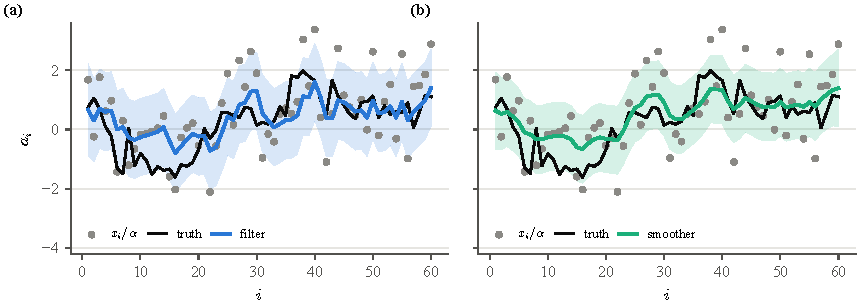
\includegraphics{primer-kalman.pdf}
\caption{A Gaussian AR(1) chain ($\rho=0.85$, black) seen through the channel at $t=0.47$ (grey dots, rescaled
by $1/\alpha$). (a) The Kalman filter mean with a two-standard-deviation band. (b) The RTS smoother: tighter, and
centred on the truth rather than lagging behind it.}
\label{fig:kalman}
\end{figure}

\subsection{What the smoother computes, and what it does not}

Everything in \eqref{eq:ssm} is jointly Gaussian, so the conditional mean is linear in the data and equals the
LMMSE estimator. Since $\Cov(a,x)=\alpha\Sigma_0$ and $\Var(x)=\alpha^2\Sigma_0+\Delta I$ with $\Sigma_0$ the clean
covariance ($\rho^{|i-j|}$),
\begin{equation}\label{eq:lmmse}
  m^s=\alpha\,\Sigma_0\big(\alpha^2\Sigma_0+\Delta I\big)^{-1}x .
\end{equation}
The smoother computes this $L$-dimensional linear solve in $O(L)$ operations instead of $O(L^3)$, by exploiting
the tridiagonal precision of the chain. Tweedie's formula \eqref{eq:tweedie} turns it into the score, and the
result is the score of the Gaussian law of $x$ itself, as it must be:
\[
  \frac{\alpha m^s-x}{\Delta}=\frac{\alpha^2\Sigma_0(\alpha^2\Sigma_0+\Delta I)^{-1}-I}{\Delta}\,x
  =\frac{\big(\alpha^2\Sigma_0-(\alpha^2\Sigma_0+\Delta I)\big)(\alpha^2\Sigma_0+\Delta I)^{-1}}{\Delta}\,x=-(\alpha^2\Sigma_0+\Delta I)^{-1}x .
\]

Now run the same recursions on a \emph{non-Gaussian} AR(1) chain, for instance with Laplace innovations of
variance $q$. The prediction step \eqref{eq:kfpredict} is still correct for the mean and variance, because the
first two moments of $\rho a+\varepsilon$ depend on $\varepsilon$ only through its mean and variance. What is lost is
everything else about the belief: its shape. Running Kalman on a non-Gaussian chain is running it on the
chain's covariance twin, and it returns \eqref{eq:lmmse} again.

\begin{inproject}
The paper's Proposition~1 makes this exact: \emph{moment-projected} belief propagation (replace every message
by the Gaussian with its mean and variance after each step, also called Gaussian closure or assumed-density
filtering) returns exactly the LMMSE estimator of the covariance twin, whatever the innovation law. So
``Gaussian closure'' and ``the linear floor'' are the same arm. On the $\phi^4$ field the projected recursion
is not even well-posed (\S\ref{sec:closurefail}), and the closure arm is the floor by definition.
\end{inproject}

\begin{caution}
The forward pass alone is the Kalman \emph{filter}; the full forward--backward computation is a
\emph{smoother}. The consolidated note asks that the two never be confused in the paper.
\end{caution}

\paragraph{Check yourself.}
\begin{enumerate}[label=\thesection.\arabic*,leftmargin=2.2em]
\item Take $P^-=1$ and the level where $\alpha^2=\Delta=\tfrac12$. Compute the gain $k$ and the filtered variance $P$.
\item Why can the smoothed variance $P_i^s$ never exceed the filtered variance $P_i$?
\end{enumerate}

\section{Hidden Markov models, Markov random fields, and belief propagation}\label{sec:bp}

\subsection{Forward and backward messages}

A \emph{hidden Markov model} is any chain \eqref{eq:chain} whose states are seen only through noisy
observations $x_i$ with likelihood $\ell_i(a)=p(x_i\mid a_i=a)$; for our channel $\ell_i(a)=\N(x_i;\alpha a,\Delta)$.
The states can be discrete (weather: sunny or rainy) or continuous (our chains). We want $p(a_i\mid x_{1:L})$
for every $i$ without integrating over all $L$ states at once. Define the forward and backward messages
\begin{equation}\label{eq:msgdef}
  \fwd_i(a)=p(x_1,\dots,x_i,\ a_i=a),\qquad \bwd_i(a)=p(x_{i+1},\dots,x_L\mid a_i=a).
\end{equation}
Splitting the sequence at site $i$ and using the Markov property,
\begin{equation}\label{eq:posterior}
  p(a_i=a\mid x_{1:L})=\frac{\fwd_i(a)\,\bwd_i(a)}{p(x_{1:L})}.
\end{equation}
Both messages obey one-step recursions. To get $\fwd_{i+1}$, sum over the value of $a_i$ (the intermediate
state), move one step with $K$, and multiply by the new likelihood:
\begin{equation}\label{eq:fwd}
  \fwd_1(a)=\mu(a)\ell_1(a),\qquad \fwd_{i+1}(a')=\ell_{i+1}(a')\int K(a'\mid a)\,\fwd_i(a)\dd a .
\end{equation}
Symmetrically, starting from $\bwd_L\equiv1$,
\begin{equation}\label{eq:bwd}
  \bwd_i(a)=\int K(a'\mid a)\,\ell_{i+1}(a')\,\bwd_{i+1}(a')\dd a' .
\end{equation}
The integrals are the matrix products \eqref{eq:matprod} on the grid: the cost is $L$ multiplications of an
$N_g$-vector by an $N_g\times N_g$ matrix, $O(LN_g^2)$, instead of the $N_g^L$ terms of brute-force summation. In
practice each message is rescaled after every step and the logarithms of the scales are accumulated, which
keeps everything in range and gives the \emph{evidence} for free:
$p(x_{1:L})=\int\fwd_L(a)\dd a$.

\begin{example}[three days of umbrellas]
A two-state chain: each day is rainy (R) or sunny (S), the weather stays the same with probability $0.8$, and
day one is R or S with probability $\tfrac12$. We never see the weather, only whether a colleague carries an
umbrella: with probability $0.9$ on a rainy day and $0.2$ on a sunny one. Over three days we see umbrella,
umbrella, no umbrella. The recursions \eqref{eq:fwd}--\eqref{eq:bwd} with sums in place of integrals give:
\begin{center}\small
\begin{tabular}{@{}lccc@{}}
\toprule
 & day 1 & day 2 & day 3 \\
\midrule
forward $(\fwd(\mathrm R),\fwd(\mathrm S))$ & $(0.450,\ 0.100)$ & $(0.342,\ 0.034)$ & $(0.0280,\ 0.0765)$ \\
backward $(\bwd(\mathrm R),\bwd(\mathrm S))$ & $(0.199,\ 0.149)$ & $(0.240,\ 0.660)$ & $(1,\ 1)$ \\
filtered $P(\mathrm R\mid\text{data so far})$ & $0.818$ & $0.910$ & $0.268$ \\
smoothed $P(\mathrm R\mid\text{all data})$ & $0.858$ & $0.785$ & $0.268$ \\
\bottomrule
\end{tabular}
\end{center}
For instance $\fwd_2(\mathrm R)=0.9\times(0.8\times0.450+0.2\times0.100)=0.342$. At every day the product
$\fwd(\mathrm R)\bwd(\mathrm R)+\fwd(\mathrm S)\bwd(\mathrm S)$ equals the same number, $0.1045$: the evidence, the probability of the
three observations. Day two shows what smoothing adds: knowing only the past, rain is $91\,\%$ likely; the dry
third day lowers it to $79\,\%$. The future revises the past, and that is the backward message's job.
\end{example}

\begin{figure}[h]\centering
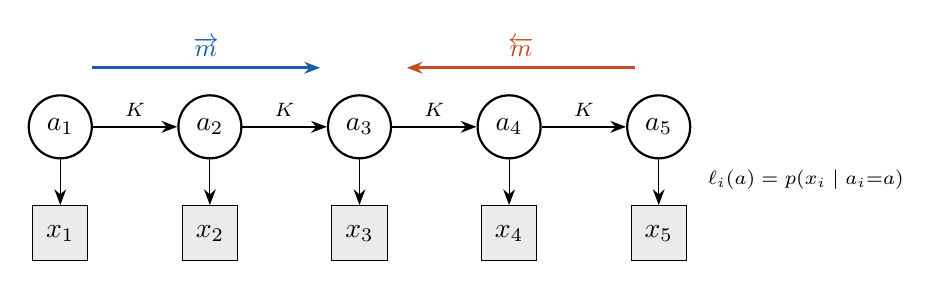
\begin{tikzpicture}[node distance=1.55cm,
  hid/.style={circle,draw,thick,minimum size=0.8cm,inner sep=0pt},
  obs/.style={rectangle,draw,fill=black!8,minimum size=0.7cm,inner sep=0pt},
  >={Stealth[length=2mm]}]
\foreach \i in {1,...,5} {
  \node[hid] (a\i) at (1.9*\i,0) {$a_{\i}$};
  \node[obs] (x\i) at (1.9*\i,-1.35) {$x_{\i}$};
  \draw[->] (a\i) -- (x\i);
}
\foreach \i/\j in {1/2,2/3,3/4,4/5} { \draw[->,thick] (a\i) -- node[above,font=\scriptsize]{$K$} (a\j); }
\draw[->,very thick,keyc] (2.3,0.75) -- node[above,font=\small]{$\fwd$} (5.2,0.75);
\draw[->,very thick,warnc] (9.2,0.75) -- node[above,font=\small]{$\bwd$} (6.3,0.75);
\node[font=\scriptsize,anchor=west] at (10.0,-0.67) {$\ell_i(a)=p(x_i\mid a_i{=}a)$};
\end{tikzpicture}
\caption{A hidden Markov chain. Forward messages carry the evidence from the left, backward messages the
evidence from the right; at each site their product is the posterior \eqref{eq:posterior}.}
\label{fig:chaingraph}
\end{figure}

\paragraph{Pair marginals.} Learning (\S\ref{sec:em}) needs the posterior of \emph{neighbouring pairs},
which the same messages give:
\begin{equation}\label{eq:pair}
  \xi_i(a,a')=p(a_i=a,a_{i+1}=a'\mid x_{1:L})=\frac{\fwd_i(a)\,K(a'\mid a)\,\ell_{i+1}(a')\,\bwd_{i+1}(a')}{p(x_{1:L})}.
\end{equation}

\paragraph{Continuous states on a grid.} Replace every integral by the weighted sum \eqref{eq:trapezoid}. The
result is \emph{exact} belief propagation for the discretised model, and the discretisation error is measured,
not assumed: on Gaussian chains the grid reproduces the closed-form smoother \eqref{eq:rts} to double
precision, and against a four-times finer grid the score changes by less than $10^{-5}$ relative on ordinary
data. When the chain is Gaussian, every message in \eqref{eq:fwd}--\eqref{eq:bwd} is a Gaussian bump and the
recursions reduce to the Kalman filter and smoother: grid BP carries $401$ numbers where $2$ would do, which is
why it is a diagnostic there and a necessity elsewhere.

\subsection{Markov random fields: the undirected view}

The same chain can be written without arrows. A \emph{Markov random field} on a graph assigns to every
configuration an energy built from local terms and sets
\begin{equation}\label{eq:mrf}
  p(a)=\frac{1}{\Zp}\exp\big(-\En(a)\big),\qquad \En(a)=\sum_{\text{edges }(i,j)}W(a_i,a_j)+\sum_iU(a_i),
\end{equation}
with $\Zp=\int e^{-\En}$ the \emph{partition function}. The pair energy $W$ rewards compatible neighbours, the
site energy $U$ favours some values. The defining property is local: given its neighbours, a site is
independent of everything else, because only the terms touching it change when it changes. (The
Hammersley--Clifford theorem says that for positive densities this local property and the factorisation
\eqref{eq:mrf} are equivalent.) A \emph{hidden} Markov random field adds noisy observations of each site;
since the likelihood is a product of site terms, the posterior is again a Markov random field with $U$
replaced by $U-\log\ell_i$. Denoising is inference in a hidden Markov random field.

On a two-dimensional grid (images) the graph has loops and exact inference is hopeless; one uses
approximations such as Besag's iterated conditional modes, Gibbs sampling (Geman and Geman) or loopy belief
propagation. On a line there are no loops, and everything is exact.

\paragraph{Transfer matrices.} On a chain, write $T(a,a')=e^{-W(a,a')-U(a)/2-U(a')/2}$ (splitting each site term
between its two bonds). Then the partition function is a product of matrices,
\[
  \Zp=\int\!\!\cdots\!\!\int T(a_1,a_2)T(a_2,a_3)\cdots T(a_{L-1},a_L)\,(\text{boundary terms}),
\]
each integral being the sum over an intermediate index in \eqref{eq:matprod}. Belief propagation, the
forward--backward algorithm and the transfer-matrix method of statistical physics are \emph{one computation in
three languages}.

\subsection{From undirected back to directed: the hidden future factor}\label{sec:futurefactor}

A chain-shaped random field is a Markov chain, but its transition kernel is \emph{not} simply $e^{-W(a,\cdot)}$
normalised. Condition on $a_i$: the law of $a_{i+1}$ is proportional to $T(a_i,a_{i+1})$ times the total weight
of all ways the chain can continue from $a_{i+1}$ to the right end, which is a backward message of the
unobserved chain. Arriving at a value from which many good continuations exist is more likely. For a long
chain this ``future factor'' becomes the leading eigenvector of $T$ (\S\ref{sec:transfer}). Keep this in mind:
it is the origin of the tilt in the tilted walk (\S\ref{sec:synthesis}).

\subsection{Belief propagation in general}

On any graph without loops (a tree), \emph{sum-product} belief propagation passes messages along edges: the
message from a node to a neighbour is the sum, over the node's value, of its local factor times the pair
factor times all messages it received from its \emph{other} neighbours. After one sweep inwards and one
outwards every node holds its exact marginal. On a chain this is \eqref{eq:fwd}--\eqref{eq:bwd}. Replacing sums
by maximisations gives \emph{max-product} (the Viterbi algorithm), which finds the single most probable
configuration rather than the posterior mean. Drawing $a_L$ from its posterior and then $a_i$ from
$p(a_i\mid a_{i+1},x)\propto\fwd_i(a_i)K(a_{i+1}\mid a_i)$ going leftwards samples whole configurations from the
posterior (forward filtering, backward sampling).

\subsection{When Gaussian closure breaks}\label{sec:closurefail}

Gaussian closure replaces each message by a Gaussian with its mean and variance. For a message that says ``the
next site is in one of two wells, $+1$ or $-1$'', the Gaussian with the same moments is a broad bump centred at
zero, on the barrier, where the field almost never is. On the $\phi^4$ chain something stronger happens: from
any value far outside the bulk, the kernel jumps straight back into the bulk, so the backward message
$\bwd_i(a)$ is nearly flat over the whole grid and its moment projection is meaningless. Measured: $38$--$43\,\%$ of
a projected message's mass sits in the outer $5\,\%$ of the grid at the base cell and $98$--$100\,\%$ on the other
cells (E32, E33 oracles). This is why the closure arm of the field experiments is the linear floor.

\paragraph{Check yourself.}
\begin{enumerate}[label=\thesection.\arabic*,leftmargin=2.2em]
\item Brute force would sum over every configuration of the hidden chain. For $L=32$ sites on a grid of $N_g=401$
  points, compare the number of terms with the cost of belief propagation.
\item In the umbrella example, recompute $\bwd_2(\mathrm R)$ from \eqref{eq:bwd} and check that
  $\fwd_2(\mathrm R)\bwd_2(\mathrm R)+\fwd_2(\mathrm S)\bwd_2(\mathrm S)$ is the evidence.
\end{enumerate}

% Part III: spectral tools (sections 7-8)
\addcontentsline{toc}{part}{Part III \quad Spectral tools}
\section{Fourier analysis: why noise erases fine detail}\label{sec:fourier}

\subsection{Waves}

A complex number is $u+iv$ with $i^2=-1$. Euler's formula $e^{i\theta}=\cos\theta+i\sin\theta$ packs a cosine and a
sine into one exponential of modulus one. The function $x\mapsto e^{ikx}$ is a \emph{wave} of frequency $k$: it
oscillates $k/2\pi$ times per unit length. Large $k$ means fast oscillation, fine detail.

The \emph{Fourier transform} decomposes a function into waves:
\begin{equation}\label{eq:ft}
  \hat f(k)=\int f(x)\,e^{-ikx}\dd x,\qquad f(x)=\frac{1}{2\pi}\int\hat f(k)\,e^{ikx}\dd k .
\end{equation}
$|\hat f(k)|$ says how much of frequency $k$ the function contains. For a density $p$, $\hat p(k)=\E[e^{-ika}]$ is
the \emph{characteristic function}, and its logarithm is the cumulant expansion of \S\ref{sec:cumulants} with
$s=-ik$. On a grid of $N_g$ points the discrete version is computed by the fast Fourier transform (FFT) in
$O(N_g\log N_g)$ operations.

\subsection{Why waves: shifts, convolutions, derivatives}

Waves are special because \emph{shifting a wave only multiplies it by a number}: $e^{ik(x-c)}=e^{-ikc}e^{ikx}$. Three
consequences follow, each in one line.
\begin{itemize}
\item \textbf{Shift.} If $g(x)=f(x-c)$ then $\hat g(k)=e^{-ikc}\hat f(k)$.
\item \textbf{Convolution.} The convolution $(f*g)(x)=\int f(y)g(x-y)\dd y$ is a weighted sum of shifted copies
  of $g$. Substituting $x=y+u$ in $\int\!\!\int f(y)g(x-y)e^{-ikx}\dd y\dd x$ splits it into
  $\int f(y)e^{-iky}\dd y\int g(u)e^{-iku}\dd u$:
  \begin{equation}\label{eq:convthm}
    \widehat{f*g}=\hat f\,\hat g .
  \end{equation}
  Convolution, which costs $O(N_g^2)$ on a grid, becomes multiplication, which costs $O(N_g)$.
\item \textbf{Derivatives.} Integrating by parts, $\widehat{f'}(k)=ik\hat f(k)$, so $\widehat{f''}(k)=-k^2\hat f(k)$. On a grid the
  second difference \eqref{eq:seconddiff} acts on a wave as
  $e^{ik(x+h)}-2e^{ikx}+e^{ik(x-h)}=-4\sin^2(kh/2)\,e^{ikx}$, i.e.\ multiplication by $-\tfrac{4}{h^2}\sin^2(kh/2)\approx-k^2$.
  Waves are the eigenfunctions of the Laplacian, with eigenvalue $-k^2$.
\end{itemize}

\subsection{Noise is a low-pass filter}

The density of a sum of independent quantities is the convolution of their densities. So for the channel
\eqref{eq:channel}, by \eqref{eq:convthm} and the Gaussian transform $\widehat{\N(0,\sigma^2)}(k)=e^{-\sigma^2k^2/2}$
(complete the square in the exponent),
\begin{equation}\label{eq:noisefourier}
  \hat p_t(k)=\hat p_0(\alpha k)\;e^{-\Delta k^2/2}.
\end{equation}
The factor $e^{-\Delta k^2/2}$ crushes high frequencies: sharp features of the clean density, such as two narrow
humps separated by a dip, are the first casualties. Figure~\ref{fig:fourier} shows it on the $\phi^4$ marginal:
its two humps are gone by $t\approx0.3$, and at $t=0.7$ the noised density is visibly a Gaussian.

\begin{figure}[h]\centering
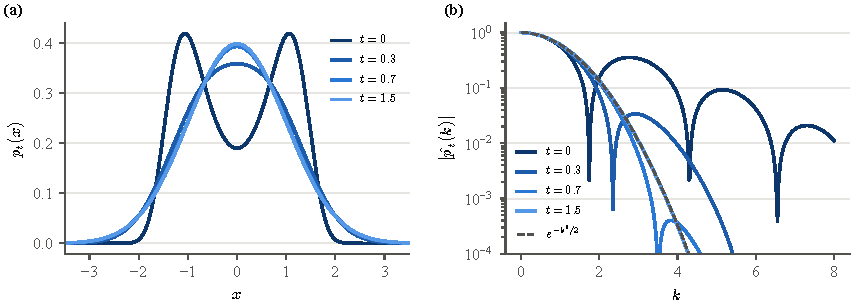
\includegraphics{primer-fourier.pdf}
\caption{(a) The standardised $\phi^4$ marginal at $\Th=0.3$, $h=1$ ($t=0$) and its noised versions. (b) The modulus
of their Fourier transforms. The clean density has strong high-frequency content (the oscillating lobes);
noise multiplies by $e^{-\Delta k^2/2}$ and leaves the Gaussian envelope $e^{-k^2/2}$ (dashed).}
\label{fig:fourier}
\end{figure}

\subsection{The heat equation}

Let $u(x,s)$ evolve by the \emph{heat equation} $\partial_su=\tfrac12\partial_x^2u$: the value at each point moves
towards the average of its neighbours, at a rate set by the second difference. In Fourier variables the
right side is $-\tfrac12k^2\hat u$, so each wave evolves on its own, $\hat u(k,s)=\hat u(k,0)e^{-k^2s/2}$. Comparing with
\eqref{eq:noisefourier}: running the heat equation for time $s$ is the same as convolving with $\N(0,s)$. The
density of a randomly walking particle obeys the heat equation, and ``adding Gaussian noise'' and ``diffusing''
are the same operation. We will meet the heat equation again as the spring term of the Allen--Cahn equation.

\subsection{Fourier and belief propagation}

The $\phi^4$ transfer kernel (\S\ref{sec:transfer}) has the form $T(\phi,\phi')=D(\phi)\,G(\phi'-\phi)\,D(\phi')$, with $G$ a
Gaussian. A message update is then: multiply by $D$ in real space, convolve with $G$ (diagonal in Fourier
space), multiply by $D$ and by the likelihood (diagonal in real space). With FFTs in between, a step costs
$O(N_g\log N_g)$ instead of $O(N_g^2)$. This was the meeting's ``Fourier BP'' idea, and the field makes it natural.
We measured that it cannot pay much at our sizes: at $N_g=401$ the dense product is a minority of the sweep
time, which is dominated by memory traffic, so the end-to-end speed-up is capped near $1.3\times$ (E24). A
truncated Fourier series of a message can also go negative, which a probability cannot.

\begin{caution}
Three spectral ideas must not be confused. \emph{Fourier modes} are a computational basis (diagonalise
convolution). \emph{Hermite modes} (next chapter) diagonalise the noising channel. \emph{Transfer-operator
eigenfunctions} (\S\ref{sec:transfer}) describe the stationary law and the correlation length of the field.
\end{caution}

\paragraph{Check yourself.}
\begin{enumerate}[label=\thesection.\arabic*,leftmargin=2.2em]
\item Why does adding independent noise $\sqrt\Delta z$ multiply the characteristic function by $e^{-\Delta k^2/2}$?
\item On a grid of spacing $h$, the fastest wave has wavelength $2h$ ($k=\pi/h$). By what factor does the second
  difference multiply it?
\end{enumerate}

\section{Hermite polynomials: why fourth-order structure fades like $e^{-4t}$}\label{sec:hermite}

\subsection{The right basis for the channel}

The channel \eqref{eq:channel} does two things: it shrinks ($a\mapsto e^{-t}a$) and it blurs (adds Gaussian noise).
Waves diagonalise blurring but not shrinking. Polynomials orthogonal with respect to the Gaussian
diagonalise both. Define the inner product $\langle f,g\rangle=\E[f(Z)g(Z)]$ for $Z\sim\N(0,1)$ and orthogonalise
$1,x,x^2,\dots$ one at a time (Gram--Schmidt). Using $\E Z^2=1$, $\E Z^4=3$, $\E Z^6=15$:
\begin{equation}\label{eq:hermite}
  H_0=1,\quad H_1=x,\quad H_2=x^2-1,\quad H_3=x^3-3x,\quad H_4=x^4-6x^2+3,\ \dots
\end{equation}
For instance $H_2=x^2-\E Z^2$ removes the part of $x^2$ along $1$, and $H_3=x^3-3x$ removes the part along
$x$ ($\E[Z^3\cdot Z]=3$). These are the (probabilists') \emph{Hermite polynomials} (Figure~\ref{fig:hermite}a). They
have a compact \emph{generating function},
\begin{equation}\label{eq:genfun}
  G(x;s)=e^{sx-s^2/2}=\sum_{n\ge0}H_n(x)\frac{s^n}{n!},
\end{equation}
from which everything follows. Orthogonality: $\E[G(Z;s)G(Z;r)]=e^{-(s^2+r^2)/2}\E e^{(s+r)Z}=e^{sr}$, and matching
powers of $sr$ gives $\E[H_mH_n]=n!$ if $m=n$ and $0$ otherwise. Differentiating \eqref{eq:genfun} in $x$ gives
$H_n'=nH_{n-1}$.

\subsection{The channel multiplies $H_n$ by $e^{-nt}$}

\begin{proposition}\label{prop:hermite}
For $f$ a function, let $(P_tf)(a)=\E\big[f(e^{-t}a+\sqrt{1-e^{-2t}}\,Z)\big]$ be the average of $f$ over the channel
started at $a$. Then $P_tH_n=e^{-nt}H_n$.
\end{proposition}
\begin{proof}
Apply $P_t$ to the generating function. With $\alpha=e^{-t}$, $\Delta=1-\alpha^2$,
\[
  P_tG(\cdot;s)(a)=\E\,e^{s\alpha a+s\sqrt\Delta Z-s^2/2}=e^{s\alpha a+s^2\Delta/2-s^2/2}=e^{(s\alpha)a-(s\alpha)^2/2}=G(a;s\alpha),
\]
because $\Delta-1=-\alpha^2$. Expanding both sides in powers of $s$: $\sum_n(P_tH_n)(a)s^n/n!=\sum_nH_n(a)\alpha^ns^n/n!$.
\end{proof}

\subsection{Densities, cumulants, and the noised law}

Write a standardised density relative to the Gaussian as
\begin{equation}\label{eq:gramcharlier}
  p(a)=\varphi(a)\Big(1+\sum_{n\ge3}c_n\frac{H_n(a)}{n!}\Big),\qquad c_n=\E_p[H_n(a)],
\end{equation}
with $\varphi$ the standard normal density; the coefficients are read off by orthogonality, and $c_1=c_2=0$ because
the law is standardised. In particular $c_3=\E a^3$ is the skewness and $c_4=\E a^4-3$ the excess kurtosis. Now
noise it. The noised quantity $x$ has $\E[H_n(x)]=\E[(P_tH_n)(a)]=e^{-nt}c_n$ by Proposition~\ref{prop:hermite}, so
\begin{equation}\label{eq:noisedgc}
  p_t(x)=\varphi(x)\Big(1+\sum_{n\ge3}c_n\,e^{-nt}\,\frac{H_n(x)}{n!}\Big).
\end{equation}
\begin{keyidea}
The channel leaves the Gaussian part alone and multiplies the $n$-th Hermite coefficient by $e^{-nt}$. Mean
information decays like $e^{-t}$, covariance like $e^{-2t}$, skewness like $e^{-3t}$, kurtosis like $e^{-4t}$
(Figure~\ref{fig:hermite}b). Fourth-order distinctions vanish under noise long before second-order ones.
\end{keyidea}

\begin{figure}[h]\centering
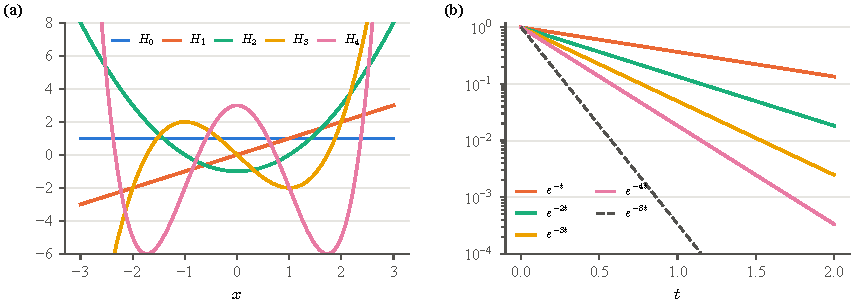
\includegraphics{primer-hermite.pdf}
\caption{(a) The Hermite polynomials $H_0,\dots,H_4$. (b) The factors $e^{-nt}$ by which the channel multiplies their
coefficients, and $e^{-8t}$, the decay of the squared non-Gaussian part of the score.}
\label{fig:hermite}
\end{figure}

\subsection{What a Gaussian denoiser misses: Theorem 2 at one site}

Take a symmetric law ($c_3=0$) and the score of \eqref{eq:noisedgc}. To first order in the small correction,
$\log p_t=\log\varphi+\log(1+R)\approx-x^2/2+R$, so using $H_n'=nH_{n-1}$,
\begin{equation}\label{eq:scorehermite}
  s_t(x)\approx-x+\sum_{n\ge3}c_n\,e^{-nt}\frac{H_{n-1}(x)}{(n-1)!}=-x+\frac{\kappa_4\,e^{-4t}}{6}\,H_3(x)+O(e^{-6t}).
\end{equation}
The covariance twin's score is exactly $-x$. Their mean-square distance is therefore
\[
  \E\big[(s_t-s_t^{\rm G})^2\big]\approx\frac{\kappa_4^2e^{-8t}}{36}\,\E[H_3^2]=\frac{\kappa_4^2}{6}\,e^{-8t}.
\]
This is the single-site version of the paper's Theorem~2, which states for a whole chain that the gap
between the exact score and the Gaussian (closure) score behaves like $\tfrac16\|\kappa_4\|_F^2e^{-8t}$, with
$\kappa_4$ the tensor of fourth cumulants across sites. On the $\phi^4$ field the ratio of the measured gap to this
prediction rises towards one with $t$ and reaches $0.73$ to $0.94$ at $t=3$ (E32, frozen).

\subsection{Many sites}

For a sequence, use products $H_{n_1}(x_1)\cdots H_{n_L}(x_L)$. The same proof shows that the channel multiplies
such a product by $e^{-(n_1+\dots+n_L)t}$. The covariance between sites $i$ and $j$ is the coefficient of
$H_1(x_i)H_1(x_j)$, degree $2$, so it survives like $e^{-2t}$; a fourth cumulant across sites has total degree
$4$ and fades like $e^{-4t}$.

\begin{caution}
Adding independent Gaussian noise $\sigma z$ to $a$ does \emph{not} change its cumulants of order $3$ and higher
(they add, and the Gaussian contributes zero). What shrinks is their size \emph{relative to the variance},
which grows. Under the variance-preserving channel the two effects are combined into the single factor
$\alpha^n=e^{-nt}$ of \eqref{eq:cumdecay}. Both descriptions say the same thing; mixing them up is a common
source of wrong exponents.
\end{caution}

\paragraph{Check yourself.}
\begin{enumerate}[label=\thesection.\arabic*,leftmargin=2.2em]
\item Check directly that $H_3$ is orthogonal to $H_1$ under the standard normal.
\item By what factor does the non-Gaussian part of the score in \eqref{eq:scorehermite} shrink between $t=0.5$ and $t=1$?
  And its squared error?
\end{enumerate}

% Part IV: learning (sections 9-10)
\addcontentsline{toc}{part}{Part IV \quad Learning}
\section{Maximum likelihood, EM, and generalised EM}\label{sec:em}

\subsection{Likelihood and its target}

A model is a family of densities $p_\theta$ indexed by parameters $\theta$. Given independent data $y_1,\dots,y_n$,
the \emph{log-likelihood} $\mathcal L(\theta)=\sum_k\log p_\theta(y_k)$ scores how well $\theta$ explains them, and
the \emph{maximum likelihood estimate} (MLE) maximises it. Two examples we use.
For a Gaussian, the MLE of the mean is the sample mean and of the variance the mean squared deviation. For
a clean AR(1) chain, $\mathcal L(\rho,q)=\sum_i\log\N(a_{i+1};\rho a_i,q)$, which is a least-squares problem:
$\hat\rho=\sum_ia_ia_{i+1}/\sum_ia_i^2$ and $\hat q$ the mean squared residual.

What does the MLE converge to? Divide $\mathcal L$ by $n$: by the law of large numbers it approaches
$\E_{\rm true}[\log p_\theta(y)]$. Compare with the \emph{Kullback--Leibler divergence}
\[
  \KL(p\,\|\,q)=\int p\log\frac pq\;\ge0,\qquad\text{with equality only if }p=q,
\]
(the inequality is Jensen's: $\E_p\log(q/p)\le\log\E_p(q/p)=\log1=0$). Since
$\E_{\rm true}\log p_\theta=-\KL(p_{\rm true}\|p_\theta)+\text{const}$, maximising likelihood is minimising the
divergence from the truth to the model.

\begin{keyidea}
If the truth is in the family, the MLE finds it (consistency). If it is not, the MLE converges to the member
\emph{closest} to the truth in KL divergence, and stays there: the remaining error is an asymptotic bias that
no amount of data removes. Separating ``needs more data'' from ``needs a better family'' is what several of our
predictions test (E33 P1, E35 P2).
\end{keyidea}

\subsection{Latent variables and the evidence lower bound}

Often the model describes a pair $(a,x)$ but we observe only $x$: the clean chain behind the noised one, the
component label behind a mixture draw. The likelihood is then the \emph{evidence}
$\log p_\theta(x)=\log\int p_\theta(x,a)\dd a$, the logarithm of an integral, awkward to maximise. The way in is a
lower bound. For \emph{any} density $q(a)$, by Jensen's inequality,
\begin{equation}\label{eq:elbo}
  \log p_\theta(x)=\log\int q(a)\frac{p_\theta(x,a)}{q(a)}\dd a\;\ge\;\int q(a)\log\frac{p_\theta(x,a)}{q(a)}\dd a=:F(q,\theta).
\end{equation}
$F$ is the \emph{evidence lower bound} (ELBO). The gap is exactly a divergence: writing
$p_\theta(x,a)=p_\theta(a\mid x)p_\theta(x)$ inside $F$ gives
\begin{equation}\label{eq:elbogap}
  \log p_\theta(x)=F(q,\theta)+\KL\big(q\,\|\,p_\theta(\cdot\mid x)\big),
\end{equation}
so the bound is tight exactly when $q$ is the posterior.

\subsection{The EM algorithm}

EM climbs $F$ by alternating over its two arguments.
\begin{itemize}
\item \textbf{E-step.} Set $q=p_{\theta_{\rm old}}(a\mid x)$, the posterior under the current parameters. By
  \eqref{eq:elbogap} this closes the gap: $F(q,\theta_{\rm old})=\log p_{\theta_{\rm old}}(x)$.
\item \textbf{M-step.} Maximise $F(q,\theta)$ over $\theta$ with $q$ fixed. The term $-\int q\log q$ does not involve
  $\theta$, so this maximises
  \begin{equation}\label{eq:Q}
    Q(\theta\mid\theta_{\rm old})=\E_{a\sim p_{\theta_{\rm old}}(\cdot\mid x)}\big[\log p_\theta(x,a)\big],
  \end{equation}
  the expected \emph{complete-data} log-likelihood.
\end{itemize}

\begin{proposition}[EM never decreases the evidence]
$\log p_{\theta_{\rm new}}(x)\ge\log p_{\theta_{\rm old}}(x)$.
\end{proposition}
\begin{proof}
$\log p_{\theta_{\rm new}}(x)\ge F(q,\theta_{\rm new})\ge F(q,\theta_{\rm old})=\log p_{\theta_{\rm old}}(x)$: the bound, then the M-step,
then the tight E-step.
\end{proof}

The proof also shows what is \emph{needed}: any $\theta_{\rm new}$ with $Q(\theta_{\rm new}\mid\theta_{\rm old})\ge Q(\theta_{\rm old}\mid\theta_{\rm old})$
works. A decrease of the evidence is therefore always a bug or a too-generous approximate step, never a feature
of EM. Our code records every decrease rather than stopping on it.

\begin{example}[a mixture of two Gaussians]
Data $y_k$ come from component $c\in\{1,2\}$ with probability $w_c$, then $y_k\sim\N(\mu_c,\sigma_c^2)$. The label is
latent. The E-step computes the \emph{responsibilities}, the posterior probabilities of the labels,
\[
  r_{kc}=\frac{w_c\,\N(y_k;\mu_c,\sigma_c^2)}{\sum_{c'}w_{c'}\,\N(y_k;\mu_{c'},\sigma_{c'}^2)};
\]
the M-step sets $w_c$ to the average responsibility and $\mu_c,\sigma_c^2$ to responsibility-weighted means and
variances. Figure~\ref{fig:em} shows the evidence rising at every iteration, with a long plateau: when the
components overlap, EM can crawl.
\end{example}

\begin{figure}[h]\centering
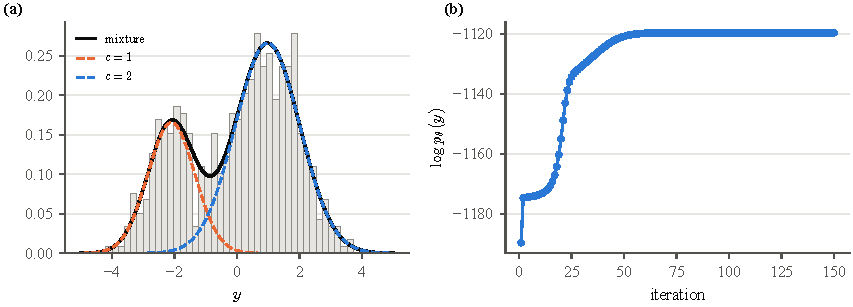
\includegraphics{primer-em.pdf}
\caption{EM on a two-component mixture ($600$ draws). (a) The fitted mixture and its components. (b) The
log-evidence per iteration: never decreasing, but slow while the components are still entangled.}
\label{fig:em}
\end{figure}

\subsection{Generalised EM: the family}

Exact E- and M-steps are luxuries. The variants keep the monotone climb by relaxing one of them.
\begin{itemize}
\item \textbf{Generalised EM (GEM).} Any parameter with higher $Q$ instead of the maximiser. Our kernels accept an
  M-step only if $Q$ did not decrease, and otherwise return the old parameters.
\item \textbf{ECM} (expectation conditional maximisation). Maximise $Q$ over blocks of parameters in turn. The
  innovation-mixture kernel updates its correlation, then its components.
\item \textbf{Gradient EM.} One or a few gradient steps on $Q$, with a line search; the neural (MDN) kernel does
  this with Adam steps and backtracking.
\item \textbf{Variational EM.} When the exact posterior is intractable (two-dimensional fields), restrict $q$ to a
  simple family and maximise $F$ over it; the bound \eqref{eq:elbo} is no longer tight, so one maximises a bound
  rather than the evidence.
\item \textbf{Monte Carlo and stochastic EM.} Replace the expectation in \eqref{eq:Q} by an average over posterior
  samples; online EM updates the expected statistics as data stream in.
\end{itemize}
All are instances of \emph{minorise--maximise}: $F(q,\cdot)$ is a function below $\log p_\theta(x)$ that touches it at
$\theta_{\rm old}$, and any increase of the minoriser is an increase of the target.

\subsection{EM on chains (Baum--Welch)}\label{sec:emchain}

For a hidden Markov chain, $\log p_\theta(x,a)=\log\mu_\theta(a_1)+\sum_i\log K_\theta(a_{i+1}\mid a_i)+\sum_i\log\ell_i(a_i)$. Taking
the posterior expectation, the only part that involves the kernel is
\begin{equation}\label{eq:Qchain}
  Q(\theta)=\iint\Xi(a,a')\,\log K_\theta(a'\mid a)\dd a\dd a'+\text{(site-one term)},\qquad
  \Xi=\sum_{\text{sequences}}\sum_i\xi_i ,
\end{equation}
with $\xi_i$ the pair marginals \eqref{eq:pair}. $\Xi(a,a')$ is the \emph{expected number of transitions} from $a$ to
$a'$, and the E-step is one forward--backward pass per sequence. The M-step is a weighted fit of the kernel to
these soft counts. With clean data the posterior is a point mass and $\Xi$ is just the histogram of observed
transitions: no E-step at all.

If the kernel is an exponential family in its parameters for each source $a$,
$\log K_\theta(a'\mid a)=\theta\cdot B(a')+c(a,a')-\log Z_\theta(a)$, then $Q$ is a linear function of $\theta$ minus a sum
of log-normalisers, hence concave, and its gradient is
\begin{equation}\label{eq:expfamgrad}
  \nabla_\theta Q=\sum_{a}\Big[\sum_{a'}\Xi(a,a')B(a')-N(a)\,\E_{K_\theta(\cdot\mid a)}[B]\Big],\qquad N(a)=\sum_{a'}\Xi(a,a'):
\end{equation}
expected statistics under the data minus expected statistics under the model, source by source. The
tilted-walk kernel of \S\ref{sec:synthesis} is of this kind.

\subsection{Fisher's identity and Boltzmann learning}\label{sec:fisherid}

\begin{proposition}[Fisher's identity]
$\nabla_\theta\log p_\theta(x)=\E_{a\sim p_\theta(\cdot\mid x)}\big[\nabla_\theta\log p_\theta(x,a)\big]$.
\end{proposition}
\begin{proof}
$\nabla p_\theta(x)=\int\nabla p_\theta(x,a)\dd a=\int p_\theta(x,a)\nabla\log p_\theta(x,a)\dd a$; divide by $p_\theta(x)$.
\end{proof}
Three uses. The gradient of the evidence costs one E-step. At a fixed point of EM the gradient of $Q$ vanishes,
so EM converges to stationary points of the evidence. And it gives Boltzmann learning: for an energy model
$p_\theta(a)=e^{-\En_\theta(a)}/\Zp_\theta$ seen through a likelihood, $\nabla\log\Zp_\theta=-\E_{p_\theta}[\nabla\En_\theta]$, so
\begin{equation}\label{eq:boltzmann}
  \nabla_\theta\log p_\theta(x)=-\underbrace{\E_{a\mid x}[\nabla\En_\theta(a)]}_{\text{positive phase}}+\underbrace{\E_{a\sim p_\theta}[\nabla\En_\theta(a)]}_{\text{negative phase}} .
\end{equation}
The positive phase pulls the energy down where the data's posterior sits; the negative phase pushes it up where
the model already puts mass. For an undirected chain both phases are pair expectations computable by transfer
matrices. For a directed kernel the negative phase becomes the per-source expectation in \eqref{eq:expfamgrad}, and
no chain-wide partition function appears.

\subsection{How fast EM goes}

Near its limit EM converges geometrically, with a rate equal to the \emph{fraction of missing information}: the
share of the complete-data information about $\theta$ that the observations do not carry (\S\ref{sec:fisher}).
When noise hides most of the clean chain, that fraction is close to one and EM needs many iterations. This is
why our EM runs a ladder of checkpoints up to $1200$ iterations, selects the checkpoint on held-out data, and
flags runs whose selected checkpoint is the last one.

\paragraph{Check yourself.}
\begin{enumerate}[label=\thesection.\arabic*,leftmargin=2.2em]
\item Why does the M-step of the mixture produce responsibility-weighted averages?
\item An approximate M-step returns parameters with a \emph{lower} $Q$ than before. What can happen to the evidence?
\end{enumerate}

\section{Fisher information, Cram\'er--Rao, and quasi-likelihood}\label{sec:fisher}

\subsection{Fisher information}

The parameter score $U_\theta(x)=\partial_\theta\log p_\theta(x)$ has mean zero at the true parameter:
$\E U=\int\partial_\theta p_\theta=\partial_\theta\int p_\theta=0$. Its variance is the \emph{Fisher information},
\begin{equation}\label{eq:fisher}
  I(\theta)=\E\big[U_\theta(x)^2\big]=-\E\big[\partial_\theta^2\log p_\theta(x)\big],
\end{equation}
the second form following by differentiating $\E U=0$ once more. It is the curvature of the expected
log-likelihood at its peak: a sharp peak means the data pin the parameter down. For $n$ independent
observations it adds up to $nI(\theta)$.

\begin{proposition}[Cram\'er--Rao]
Any unbiased estimator $\hat\theta$ of $\theta$ from $n$ observations has $\Var(\hat\theta)\ge1/\big(nI(\theta)\big)$.
\end{proposition}
\begin{proof}
Differentiate $\E_\theta\hat\theta=\theta$: $\int\hat\theta\,\partial_\theta p_\theta=1$, i.e.\ $\Cov(\hat\theta,U)=1$ for the total score $U$, whose
variance is $nI$. By Cauchy--Schwarz, $1=\Cov(\hat\theta,U)^2\le\Var(\hat\theta)\,nI(\theta)$.
\end{proof}
The MLE attains the bound for large $n$: $\sqrt n(\hat\theta-\theta)$ becomes Gaussian with variance $1/I(\theta)$. With
several parameters $I$ is a matrix and the bound is its inverse.

\begin{example}[AR(1)]
With the innovation variance $q$ known, $\partial_\rho\log\N(a';\rho a,q)=(a'-\rho a)a/q$, whose mean square under the
stationary chain is $\E[\varepsilon^2]\E[a^2]/q^2=1/q$. So each clean transition carries information $1/(1-\rho^2)$ about
$\rho$, and $\Var\hat\rho\approx(1-\rho^2)/n$ from $n$ transitions.
\end{example}

\subsection{Information lost to noise}

When only noised data are seen, Fisher's identity says the observed score is the posterior average of the
complete-data score, $U_{\rm obs}=\E[U_{\rm complete}\mid x]$. The law of total variance then splits the information:
\begin{equation}\label{eq:missinginfo}
  I_{\rm complete}=I_{\rm obs}+\underbrace{\E\big[\Var(U_{\rm complete}\mid x)\big]}_{I_{\rm missing}},
\end{equation}
the \emph{missing information principle}. Noise moves information from the first term to the second.

The channel does this selectively, and Hermite polynomials say how. A parameter that changes only the
degree-$n$ Hermite content of the law enters the noised density \eqref{eq:noisedgc} through $c_ne^{-nt}$. Its score
is then about $e^{-nt}(\partial_\theta c_n)H_n(x)/n!$, and its information about $e^{-2nt}(\partial_\theta c_n)^2/n!$. A
covariance coordinate (degree $2$) loses information like $e^{-4t}$; a shape coordinate such as the kurtosis
(degree $4$) like $e^{-8t}$. Since the number of sequences needed for a fixed accuracy is inversely
proportional to the information, it grows like $e^{4t}$ and $e^{8t}$ respectively.

\begin{inproject}
E12b measured exactly this (frozen 1 October): the sample size needed for a fixed accuracy grows with the
noise level with log-slope $4.95$ (interval $3.09$ to $6.83$) for the covariance coordinate, and for the shape
coordinate the requirement is unresolved beyond $t=0.8$ even at $8192$ sequences (slope above $6.7$). Both agree
with the exact information curve, whose local slopes on these levels are $3.8$--$3.9$ and $6.1$--$6.9$; the
asymptotic $4$ and $8$ are reached only at larger $t$.
\end{inproject}

\subsection{Quasi-likelihood: using a wrong model on purpose}

Sometimes we maximise a likelihood we know to be wrong because it is convenient. This is sound if the
\emph{estimating equation} is right. Let $g(\theta)$ be the gradient of the convenient objective. If its mean
under the \emph{true} law vanishes at the target value $\theta^\star$, the solution of $g(\hat\theta)=0$ converges to
$\theta^\star$, with variance given by the \emph{sandwich} $A^{-1}BA^{-1}$, where $A=-\E[\partial g]$ and $B=\Var g$. When the
objective is the true log-likelihood, $A=B=I$ (the information equality) and the sandwich reduces to the
Cram\'er--Rao bound. When the model is simply misspecified, the MLE converges to the KL projection of the
truth (White's theorem) and the sandwich gives honest error bars around it.

The quasi-likelihood that matters here is the Gaussian one. For a zero-mean sequence with model covariance
$\Sigma_\theta$,
\[
  \ell(\theta)=-\tfrac12\log\det\Sigma_\theta-\tfrac12x\T\Sigma_\theta^{-1}x,\qquad
  \E_{\rm true}\,\ell(\theta)=-\tfrac12\log\det\Sigma_\theta-\tfrac12\operatorname{tr}\big(\Sigma_\theta^{-1}\Sigma^\star\big).
\]
It depends on the data only through their covariance, and its expectation is maximised at $\Sigma_\theta=\Sigma^\star$
whatever the true law is. A Gaussian model is therefore consistent for everything the covariance determines
(the correlation, the variance) and blind to everything else.

\begin{keyidea}
Fitting a Gaussian-innovation kernel by EM on noised chains is a Gaussian quasi-likelihood: it converges to
the covariance twin and its denoiser lands on the linear floor, never below it. To beat the floor, the kernel
family must be able to represent non-Gaussian structure. That is why the project's estimator uses mixture,
tilted and pair-energy kernels.
\end{keyidea}

\subsection{Pseudo-likelihood: avoiding the partition function}

For a Markov random field the likelihood needs $\Zp_\theta$, an integral over all configurations. Besag's
\emph{pseudo-likelihood} replaces the joint density by the product of each site's conditional law given its
neighbours, $\prod_ip_\theta(a_i\mid a_{i-1},a_{i+1})$; each factor is normalised over one site only, so no $\Zp_\theta$
appears. It is consistent but less efficient; composite likelihoods generalise it. On a chain the
exact likelihood is no harder: written with a directed kernel \eqref{eq:chain}, it needs only one normaliser per
source value, because the ground-state transform (\S\ref{sec:transfer}) has absorbed the partition function. This
is the special luck of one dimension that the learned pair energy exploits.

\paragraph{Check yourself.}
\begin{enumerate}[label=\thesection.\arabic*,leftmargin=2.2em]
\item For $n$ draws from $\N(\mu,1)$, what is the Fisher information about $\mu$, and which estimator attains the
  Cram\'er--Rao bound?
\item Why can a Gaussian quasi-likelihood never learn the kurtosis of the innovations?
\end{enumerate}

% Part V: physics (sections 11-12)
\addcontentsline{toc}{part}{Part V \quad Physics}
\section{From a ball in a valley to the stochastic Allen--Cahn equation}\label{sec:allencahn}

\subsection{Rolling downhill}\label{sec:langevin}

Picture a ball in thick honey on a landscape of height $V(x)$. It has no inertia: its velocity is the force,
\begin{equation}\label{eq:gradflow}
  \frac{\dd x}{\dd s}=-V'(x),
\end{equation}
where $s$ is time. This is a \emph{gradient flow}. Along it the height only goes down,
$\frac{\dd}{\dd s}V(x(s))=V'(x)\frac{\dd x}{\dd s}=-V'(x)^2\le0$, and the ball stops at a bottom. Our landscape is the
\emph{double well}
\begin{equation}\label{eq:doublewell}
  V(x)=\tfrac14(x^2-1)^2,
\end{equation}
with two valleys at $x=\pm1$ (height $0$) and a barrier at $x=0$ of height $1/4$ (Figure~\ref{fig:langevin}a).

\subsection{Adding random kicks}

Now let the honey be warm, so that molecules kick the ball at random. A \emph{Brownian motion} $W(s)$ is the
limit of a random walk with ever smaller, ever more frequent steps: its increments over disjoint time
intervals are independent and $W(s+\delta)-W(s)\sim\N(0,\delta)$. Its variance grows linearly with time, so its
displacement grows like $\sqrt\delta$, much faster than $\delta$ for small $\delta$ (this is why its paths are rough).
The \emph{Langevin equation} adds kicks of strength set by a \emph{temperature} $\Th$:
\begin{equation}\label{eq:langevin}
  \dd x=-V'(x)\dd s+\sqrt{2\Th}\,\dd W,\quad\text{meaning}\quad x_{n+1}=x_n-V'(x_n)\,\delta+\sqrt{2\Th\delta}\;z_n
\end{equation}
for small time steps $\delta$ and independent standard normal $z_n$. At low temperature the ball rattles in one
valley and only rarely jumps the barrier; the typical waiting time grows like $e^{\Delta V/\Th}$ with $\Delta V$ the
barrier height (the Arrhenius law). Figure~\ref{fig:langevin}b shows the hops at $\Th=0.15$.

\subsection{Where the ball spends its time}

Release many independent balls and follow their density $p(x,s)$. Probability is conserved, so the density
in an interval changes only by what flows across its ends: $\partial_sp=-\partial_xJ$, with $J$ the
\emph{probability current}. Two things make probability flow. The drift carries density $p$ at velocity $-V'$,
a current $-V'p$. The kicks spread it from crowded to empty places, a current $-\Th\,\partial_xp$ (Fick's law;
the coefficient $\Th$ is fixed by matching the spread of $\sqrt{2\Th}W$ with the heat equation of \S\ref{sec:fourier}).
Hence the \emph{Fokker--Planck equation}
\begin{equation}\label{eq:fp}
  \partial_sp=\partial_x\big(V'p\big)+\Th\,\partial_x^2p .
\end{equation}
At equilibrium nothing flows, $J=0$, i.e.\ $\Th p'=-V'p$, whose solution is
\begin{equation}\label{eq:gibbs1}
  \pi(x)=\frac{1}{\Zp}\,e^{-V(x)/\Th}.
\end{equation}
This is the \emph{Boltzmann--Gibbs} law: low energy is likely, and temperature sets how much the law cares
about energy (Figure~\ref{fig:langevin}c). The zero-current condition is the continuous form of detailed
balance \eqref{eq:detbal}: the Langevin dynamics is reversible.

\begin{figure}[h]\centering
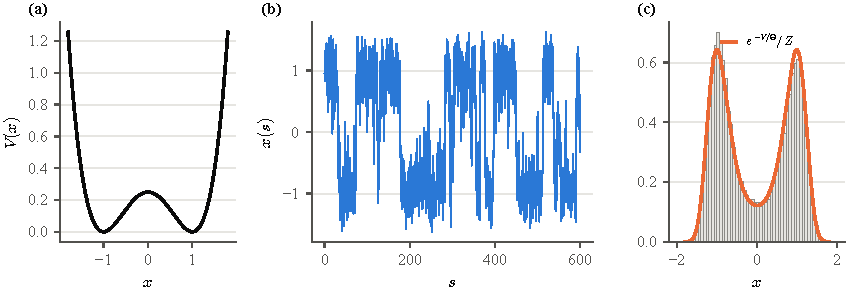
\includegraphics{primer-langevin.pdf}
\caption{(a) The double well $V$. (b) A Langevin path at $\Th=0.15$: long stays in a valley, rare hops. (c) The
histogram of the path against the Gibbs law $e^{-V/\Th}/\Zp$.}
\label{fig:langevin}
\end{figure}

\begin{keyidea}
The noising channel is a Langevin equation. With $V(x)=x^2/2$ and $\Th=1$, \eqref{eq:langevin} is the
Ornstein--Uhlenbeck process $\dd x=-x\dd s+\sqrt2\dd W$. Multiplying by $e^s$ gives $\dd(e^sx)=\sqrt2e^s\dd W$, so
started at $a$, $x(t)=e^{-t}a+\sqrt2\int_0^te^{-(t-r)}\dd W(r)$, a Gaussian with variance $2\int_0^te^{-2(t-r)}\dd r=1-e^{-2t}$.
That is exactly \eqref{eq:channel}. Its Gibbs law is $e^{-x^2/2}$, the standard normal, which is why pure noise
is where the channel ends.
\end{keyidea}

\subsection{From one ball to a string: where the Laplacian comes from}

Now take many balls, one at each point $x_i=ih$ of a line with spacing $h$, and call the value at point $i$
$\phi_i$ (think of $\phi_i$ as the local magnetisation, or the local composition of an alloy). Each $\phi_i$ sits in
its own double well, and neighbours are joined by springs that dislike differences. The total energy is
\begin{equation}\label{eq:latticeenergy}
  \En_h(\phi)=\sum_i\Big[\frac{(\phi_{i+1}-\phi_i)^2}{2h}+h\,V(\phi_i)\Big].
\end{equation}
The factors of $h$ make each piece represent a length $h$ of string: the spring term approximates
$\int\frac12(\partial_x\phi)^2\dd x$ and the well term $\int V(\phi)\dd x$. The derivative of $\En_h$ with respect to one value is
\[
  \frac{\partial\En_h}{\partial\phi_i}=-\frac{\phi_{i+1}-2\phi_i+\phi_{i-1}}{h}+h\,V'(\phi_i),
\]
and the second difference \eqref{eq:seconddiff} has appeared on its own: \emph{the springs pull each value towards
the average of its neighbours}. The gradient flow of the string, with each bead's force divided by the length
$h$ it represents, is
\begin{equation}\label{eq:latticeAC}
  \frac{\dd\phi_i}{\dd s}=\frac{\phi_{i+1}-2\phi_i+\phi_{i-1}}{h^2}-V'(\phi_i).
\end{equation}
As $h\to0$ the values become a function $\phi(x,s)$ of position and time (a \emph{field}; ``scalar'' only says
that its value at each point is a single number), the second difference becomes the second derivative in
space, and we get the \emph{Allen--Cahn equation}
\begin{equation}\label{eq:allencahn}
  \partial_s\phi=\partial_x^2\phi-V'(\phi).
\end{equation}
It is a \emph{partial differential equation} (PDE): an equation for a function of two variables involving its
derivatives in both. Two forces compete. The spring term is the heat equation: it smooths, pulling every
point towards its neighbours. The well term pushes every point towards $+1$ or $-1$. Allen and Cahn wrote it in
1979 for the separation of an alloy into regions of two phases.

\subsection{Kinks}

Where the field must change from $-1$ to $+1$ it forms a \emph{kink}. A kink at rest solves
\eqref{eq:allencahn} with $\partial_s\phi=0$: $\phi''=V'(\phi)$. Multiply by $\phi'$; the left side is the derivative of
$\tfrac12\phi'^2$ and the right side the derivative of $V(\phi)$, so $\tfrac12\phi'^2=V(\phi)$ (both vanish far from the
kink). Hence $\phi'=\sqrt{2V(\phi)}=(1-\phi^2)/\sqrt2$, which integrates to
\begin{equation}\label{eq:kink}
  \phi_{\rm kink}(x)=\tanh\big(x/\sqrt2\big),\qquad
  E_{\rm kink}=\int\Big[\tfrac12\phi'^2+V(\phi)\Big]\dd x=\int_{-1}^{1}\sqrt{2V(\phi)}\dd\phi=\frac{2\sqrt2}{3}\approx0.94 .
\end{equation}
The kink has width about $\sqrt2$ and costs a fixed energy $E_{\rm kink}$ (Figure~\ref{fig:field}a). A field made of
long stretches near $+1$ or $-1$ (\emph{domains}) separated by kinks is the typical low-temperature picture.

\subsection{Adding noise everywhere: the stochastic Allen--Cahn equation}

Heat the string: give every bead its own independent kicks, with strength scaled so that each piece of
string of length $h$ receives the right amount,
\begin{equation}\label{eq:sac}
  \dd\phi_i=\Big[\frac{\phi_{i+1}-2\phi_i+\phi_{i-1}}{h^2}-V'(\phi_i)\Big]\dd s+\sqrt{\frac{2\Th}{h}}\,\dd W_i .
\end{equation}
As $h\to0$ this is the \emph{stochastic} Allen--Cahn equation $\partial_s\phi=\partial_x^2\phi-V'(\phi)+\sqrt{2\Th}\,\eta$, with $\eta$
``space-time white noise'' (independent kicks at every point and every time). A PDE with random forcing is a
\emph{stochastic PDE}, an SPDE. In one space dimension this one is well defined: its solutions are continuous
but rough, like a Brownian path.

Where does the string spend its time? Exactly as for one ball. For any system $\dd X=-M\nabla\En\dd s+\sqrt{2\Th M}\dd W$
with a positive mobility $M$ ($M=1/h$ here), setting every component of the probability current to zero gives
\begin{equation}\label{eq:gibbsfield}
  p(\phi_1,\dots,\phi_L)\propto e^{-\En_h(\phi)/\Th}=\prod_i\exp\!\Big(-\frac{(\phi_{i+1}-\phi_i)^2}{2\Th h}\Big)\prod_i\exp\!\Big(-\frac{h\,V(\phi_i)}{\Th}\Big).
\end{equation}
\begin{keyidea}
The stationary law of the stochastic Allen--Cahn field on a lattice is \eqref{eq:gibbsfield}: a Gaussian random walk
in space (each step $\phi_{i+1}-\phi_i$ has variance $\Th h$) reweighted at every site by $e^{-hV(\phi_i)/\Th}$. Every factor
couples at most two neighbours. So by \S\ref{sec:bp} the spatial snapshot is a Markov random field on a line,
hence a Markov chain in the site index, and its exact denoiser is computable by belief propagation. We never
need to simulate the time dynamics \eqref{eq:sac}: the stationary law is all the data are drawn from.
\end{keyidea}

Two features of the lattice matter later. Each single step is \emph{nearly Gaussian} when $h$ is small, because
the reweighting factor $e^{-hV/\Th}$ is close to one; the non-Gaussian structure accumulates over the number of
sites spanned by a correlation length. And a fixed physical length contains more sites as $h$ shrinks, so a
denoiser that looks at a fixed number of neighbours sees a shrinking piece of physics.

\paragraph{Check yourself.}
\begin{enumerate}[label=\thesection.\arabic*,leftmargin=2.2em]
\item Verify that $\tanh(x/\sqrt2)$ solves $\phi''=V'(\phi)=\phi^3-\phi$.
\item What is the Gibbs law \eqref{eq:gibbs1} of the Langevin equation with $V(x)=x^2/2$ at temperature $\Th$?
\end{enumerate}

\section{The transfer operator: the field as a Markov chain}\label{sec:transfer}

\subsection{The transfer kernel and its spectrum}

Split each site factor of \eqref{eq:gibbsfield} evenly between the two bonds that touch it. The law becomes a
product of identical symmetric factors
\begin{equation}\label{eq:transfer}
  \mathsf T(\phi,\phi')=D(\phi)\,G(\phi'-\phi)\,D(\phi'),\qquad D(\phi)=e^{-hV(\phi)/2\Th},\quad G(u)=e^{-u^2/2\Th h}.
\end{equation}
Read $\mathsf T$ as an integral operator, $(\mathsf Tf)(\phi)=\int\mathsf T(\phi,\phi')f(\phi')\dd\phi'$; on a grid it is a symmetric matrix with
positive entries. By \S\ref{sec:toolbox} it has real eigenvalues $\lambda_0>\lambda_1\ge\lambda_2\ge\dots$, orthonormal
eigenfunctions $\psi_0,\psi_1,\dots$, and (Perron--Frobenius) a leading eigenfunction $\psi_0$ that is positive
everywhere. Integrating a long chain is applying $\mathsf T$ many times, so $\lambda_0$ and $\psi_0$ dominate.

\subsection{The ground-state transform}

Consider a site deep inside a long chain. Its marginal is the product of what the left half and the right half
say about it. Each half is $\mathsf T$ applied many times to the constant function at the far end, which by the power
method is proportional to $\psi_0$. So the stationary marginal is
\begin{equation}\label{eq:psi0sq}
  \pi(\phi)=\psi_0(\phi)^2\qquad(\textstyle\int\psi_0^2=1).
\end{equation}
Given the current site, the next one is drawn in proportion to the bond factor times everything to its
right, $\mathsf T(\phi,\phi')\psi_0(\phi')$ (the ``future factor'' of \S\ref{sec:futurefactor}). Normalising with the
eigen-equation $\int\mathsf T(\phi,\phi')\psi_0(\phi')\dd\phi'=\lambda_0\psi_0(\phi)$ gives the transition kernel
\begin{equation}\label{eq:gst}
  \boxed{\;K(\phi'\mid\phi)=\frac{\mathsf T(\phi,\phi')\,\psi_0(\phi')}{\lambda_0\,\psi_0(\phi)}\;}
\end{equation}
the \emph{ground-state transform} (the name comes from quantum mechanics, where $\psi_0$ is the lowest-energy
state). It is reversible with respect to $\pi=\psi_0^2$: $\pi(\phi)K(\phi'\mid\phi)=\psi_0(\phi)\mathsf T(\phi,\phi')\psi_0(\phi')/\lambda_0$ is
symmetric. Intuitively, $\psi_0(\phi')$ counts the good continuations available after arriving at $\phi'$.

\subsection{Correlations, and why there is no phase transition}

Insert the expansion $\mathsf T^r=\sum_n\lambda_n^r\psi_n\psi_n\T$ into the two-point function:
\begin{equation}\label{eq:corr}
  \E[\phi_i\,\phi_{i+r}]=\sum_{n\ge1}\Big(\frac{\lambda_n}{\lambda_0}\Big)^rc_n^2,\qquad c_n=\int\psi_0(\phi)\,\phi\,\psi_n(\phi)\dd\phi
\end{equation}
(the $n=0$ term is the squared mean, zero by symmetry). Correlations decay geometrically, dominated by
$\rho_1=\lambda_1/\lambda_0$, which plays the role of the AR(1) coefficient $\rho$: the correlation length is
$\xi=1/\log(\lambda_0/\lambda_1)$ sites. We fix the laboratory's second-order structure by choosing $h$ so that
$\rho_1=0.85$, the same value as the AR(1) laboratory.

Because $\lambda_0$ is strictly larger than $\lambda_1$ at every temperature, $\xi$ is finite: a one-dimensional system
never commits to one phase over an infinite length. The reason is entropy. A kink costs $E_{\rm kink}$ but can be
placed anywhere, so a long stretch always contains some, at a density that behaves like $e^{-E_{\rm kink}/\Th}$. The
domains are therefore long but finite, of length about $e^{E_{\rm kink}/\Th}$: a sharp crossover, not a phase
transition. Our frozen measurements (E32's fixed-spacing sweep) show coarse kink densities of $0.016$ and $0.066$
per unit length at $\Th=0.2$ and $0.3$, a ratio of $4.1$, against the Arrhenius ratio $e^{E_{\rm kink}(1/0.2-1/0.3)}=4.8$.

\begin{figure}[h]\centering
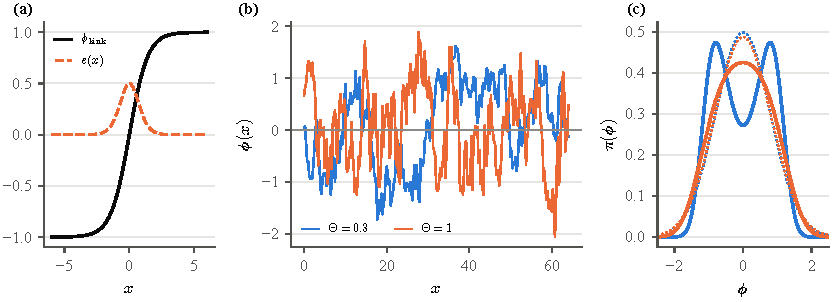
\includegraphics{primer-field.pdf}
\caption{(a) The kink $\tanh(x/\sqrt2)$ and its energy density, which integrates to $E_{\rm kink}=2\sqrt2/3$. (b) Exact
stationary fields at $h=0.25$ over a length of $64$: at $\Th=0.3$ (blue) long domains near $\pm1$ separated by kinks; at
$\Th=1$ (orange) a rough field that rarely settles. (c) The stationary marginal $\pi=\psi_0^2$ (solid) against the
Gaussian with the same variance (dotted): bimodal at $\Th=0.3$, already close to Gaussian at $\Th=1$.}
\label{fig:field}
\end{figure}

\subsection{Exact sampling and the numerics}

Since the chain is stationary with known $\pi$ and $K$, exact samples need no simulation in time: draw
$\phi_1\sim\pi$, then each next site from $K$. In the code, $\mathsf T$ is discretised on $2401$ points over $[-12,12]$, the
symmetric matrix $W^{1/2}\mathsf TW^{1/2}$ is diagonalised once per $(\Th,h)$, $\log\psi_0$ is interpolated by a spline,
and the field is standardised to unit variance, $a=\phi/s$ with $s^2=\Var_\pi\phi$, before the noise channel is applied.
The draw from $K$ is done by rejection: propose a Gaussian step of variance $\Th h$ and accept with probability
proportional to $\psi_0(\phi')D(\phi')$, a fact that the next chapter turns into a theorem.

\begin{caution}
The number of sign changes of a sampled field is \emph{not} its number of kinks. A rough path that crosses zero
once tends to recross it many times nearby, and on a finer lattice those recrossings multiply: the raw
sign-change density grows like $1/\sqrt h$ (measured: $0.120$, $0.175$, $0.247$ per unit length at $h=1,0.5,0.25$; N-31).
Counting only crossings that survive over a kink width ($\sqrt2$ in physical units) gives a statistic that agrees
across lattices within $11\,\%$, and across subsampling strides of one fine field within $8\,\%$ (E34, E36).
\end{caution}

\paragraph{Check yourself.}
\begin{enumerate}[label=\thesection.\arabic*,leftmargin=2.2em]
\item Check that the kernel \eqref{eq:gst} integrates to one over $\phi'$.
\item If $\lambda_1/\lambda_0=0.85$, after how many sites has the leading term of the correlation fallen below $0.1$ of its
  starting value?
\end{enumerate}

% Part VI: the new theory (section 13) and appendices
\addcontentsline{toc}{part}{Part VI \quad The new theory}
\section{Putting it together: the tilted walk and the learned pair energy}\label{sec:synthesis}

\subsection{The question, restated with everything we now have}

We observe many short sequences $x_{1:L}$, each a stationary snapshot of the $\phi^4$ field (\S\ref{sec:allencahn}),
standardised and passed through the channel \eqref{eq:channel} at some level $t$. We want the exact score
\eqref{eq:tweedie} at every level, which by Tweedie is the posterior mean, which by \S\ref{sec:bp} is one
forward--backward pass \emph{if we know the kernel $K$}. So the whole problem is to \emph{learn the local law}
from noised data (EM, \S\ref{sec:em}) and let belief propagation compose it exactly. The theory below says which
families of local laws can contain the truth, what their parameters mean, and why the simpler alternatives fail.

\subsection{The tilted-walk identity}

\begin{proposition}[the field's kernel is a tilted random walk]\label{prop:tilt}
With $g=\psi_0D$, the ground-state kernel \eqref{eq:gst} can be written
\begin{equation}\label{eq:tiltedwalk}
  K(\phi'\mid\phi)=\frac{\N(\phi';\phi,\Th h)\;g(\phi')}{Z_g(\phi)},\qquad Z_g(\phi)=\int\N(\phi';\phi,\Th h)\,g(\phi')\dd\phi'=\frac{\lambda_0\psi_0(\phi)}{c\,D(\phi)},
\end{equation}
with $c=\sqrt{2\pi\Th h}$ the Gaussian's normalising constant.
\end{proposition}
\begin{proof}
Insert \eqref{eq:transfer} into \eqref{eq:gst}: $K=D(\phi)G(\phi'-\phi)D(\phi')\psi_0(\phi')/(\lambda_0\psi_0(\phi))=G(\phi'-\phi)g(\phi')\cdot D(\phi)/(\lambda_0\psi_0(\phi))$. The
eigen-equation $\int\mathsf T(\phi,\phi')\psi_0(\phi')\dd\phi'=\lambda_0\psi_0(\phi)$ reads $D(\phi)\int G(\phi'-\phi)g(\phi')\dd\phi'=\lambda_0\psi_0(\phi)$, which is the
normaliser. Replace $G$ by $c\,\N(\cdot;\phi,\Th h)$.
\end{proof}

In words: \emph{take a Gaussian random-walk step of variance $\Th h$, then tilt the landing point by a positive weight
$g(\phi')$, and renormalise}. The weight combines the local preference $D(\phi')=e^{-hV(\phi')/2\Th}$ with the future factor
$\psi_0(\phi')$. The normaliser $Z_g$ is the ground-state transform itself, so a model that parametrises $\log g$ and
normalises each column numerically contains the truth \emph{without ever computing $\psi_0$ or $\lambda_0$}. In
standardised units $a=\phi/s$ the step variance is $\gamma=\Th h/s^2$.

\subsection{Where the two laboratories meet, and where they part}

\begin{proposition}\label{prop:embed}
The Gaussian AR(1) kernel $\N(a';\rho a,q)$ with $0<\rho<1$ is a tilted walk, with $\gamma=q/\rho$ and the quadratic tilt
$\log g(a')=-(1-\rho)a'^2/2q$. No other AR(1) kernel $k(a'-\rho a)$ is a tilted walk.
\end{proposition}
\begin{proof}
For the first claim, complete the square: $\N(a';a,\gamma)e^{-ca'^2}$ is a Gaussian in $a'$ with mean $a/(1+2c\gamma)$ and
variance $\gamma/(1+2c\gamma)$; setting these to $\rho a$ and $q$ gives $\gamma=q/\rho$ and $2c=(1-\rho)/q$. For the second, note
that for any tilted walk the mixed derivative $\partial_a\partial_{a'}\log K=1/\gamma$ is a constant: $\log g$ depends only on
$a'$, $\log Z_g$ only on $a$, and the Gaussian contributes $aa'/\gamma$. For $k(a'-\rho a)$ the mixed derivative is
$-\rho(\log k)''(a'-\rho a)$, constant only if $\log k$ is quadratic, i.e.\ $k$ Gaussian.
\end{proof}

So the first laboratory (AR(1) chains with non-Gaussian innovations) and the second (gradient fields like
$\phi^4$) share exactly one member, the Gaussian chain. What separates them is the \emph{drift}:

\begin{proposition}[the drift is the gradient of the log-normaliser]
For a tilted walk, $\E[a'-a\mid a]=\gamma\,(\log Z_g)'(a)$.
\end{proposition}
\begin{proof}
$Z_g'(a)=\int\partial_a\N(a';a,\gamma)\,g(a')\dd a'=\int\frac{a'-a}{\gamma}\N(a';a,\gamma)g(a')\dd a'=Z_g(a)\,\E[a'-a\mid a]/\gamma$.
\end{proof}
For the field, $\log Z_g=\log\psi_0+hV/2\Th+\text{const}$ (physical units), so the expected step is
$\Th h(\log\psi_0)'(\phi)+\tfrac{h^2}{2}V'(\phi)$: a \emph{nonlinear} function that pushes the field back towards the wells.
In the limit of small $h$ the spatial profile obeys $\dd\phi=\Th(\log\psi_0)'(\phi)\dd x+\sqrt\Th\,\dd B$: the drift in space is the
log-derivative of the ground state, not $-V'$. An AR(1) kernel with any innovation law, including the paper's
mixture of Gaussians, has a \emph{linear} drift $\rho a$. It is misspecified on the field through its drift, not
through the shape of its noise, and no amount of data repairs that (\S\ref{sec:em}).

\subsection{Every tilted walk is reversible}

\begin{proposition}[reversibility and the site energy]\label{prop:rev}
For any $\gamma>0$ and positive $g$ with finite $Z_g$, the tilted walk $K_g(a'\mid a)=\N(a';a,\gamma)g(a')/Z_g(a)$ is
reversible with invariant density $\pi_g\propto g\,Z_g$. Equivalently, it is the Gibbs chain of the symmetric pair energy
\begin{equation}\label{eq:pairenergy}
  W(a,a')=\frac{(a'-a)^2}{2\gamma}+f(a)+f(a'),\qquad f=-\tfrac12\log\big(g/Z_g\big),
\end{equation}
and conversely every pair energy of this form is a tilted walk. For the $\phi^4$ field, $f(a)=\tfrac{h}{2\Th}V(sa)+\text{const}$.
\end{proposition}
\begin{proof}
$\pi_g(a)K_g(a'\mid a)\propto g(a)Z_g(a)\N(a';a,\gamma)g(a')/Z_g(a)=g(a)g(a')\N(a';a,\gamma)$, which is symmetric in $(a,a')$: detailed
balance \eqref{eq:detbal}, hence invariance. For the second form, take $u=\sqrt{g/Z_g}=e^{-f}$ and the symmetric operator
$\mathsf T_g(a,a')=u(a)\N(a';a,\gamma)u(a')$. Then $\psi=\sqrt{gZ_g}$ satisfies $\mathsf T_g\psi=u\int\N g=uZ_g=\psi$ (using $u\psi=g$), so $\psi$ is
its Perron eigenfunction with eigenvalue $1$, and its ground-state transform is
$\mathsf T_g(a,a')\psi(a')/\psi(a)=\N(a';a,\gamma)g(a')/Z_g(a)=K_g$. The converse is Proposition~\ref{prop:tilt} with $D=e^{-f}$. For the
field, $g/Z_g=c\,D^2/\lambda_0$ by \eqref{eq:tiltedwalk}, so $f=-\log D+\text{const}=hV/2\Th+\text{const}$.
\end{proof}

\begin{keyidea}
A learned transition kernel of this form and a learned symmetric pair energy are \emph{one model}. Nothing
irreversible can be learned by mistake, and a fitted kernel \emph{reads as physics}: since $\gamma=\Th h/s^2$ and
$f(a)=\tfrac{h}{2\Th}V(sa)+\text{const}$,
\begin{equation}\label{eq:readout}
  \hat\Th=\hat\gamma\,s^2/h,\qquad\hat V(\phi)=\frac{2\hat\Th}{h}\,\hat f(\phi/s)+\text{const}.
\end{equation}
The temperature is read from the bond variance alone, the potential (its barrier, its wells) from the site
energy. Numerically, on the $401$-point grid: $\pi_g$ by formula and by eigensolve agree to $4\times10^{-12}$,
detailed balance holds to $10^{-14}$, and the field's own site energy equals $\tfrac h{2\Th}V$ to $2\times10^{-10}$.
\end{keyidea}

\subsection{Three ways to learn the local law}

\begin{enumerate}
\item \textbf{The innovation mixture} (the paper's estimator): $K(a'\mid a)=\sum_cw_c\N(a';\rho a+\mu_c,s_c^2)$, $25$ parameters at
  $8$ components. Exact on the AR(1) laboratory, misspecified on the field (linear drift).
\item \textbf{A tilt basis}: $\log g=\sum_m\theta_mB_m$ with Legendre polynomials ($7$ parameters) or cubic B-splines ($25$),
  plus $\log\gamma$. For each source value the kernel is an exponential family in $\theta$, so the M-step is concave and its
  gradient is \eqref{eq:expfamgrad}: posterior transition statistics minus the kernel's own conditional expectations,
  which is Boltzmann learning without a partition function.
\item \textbf{The site energy itself} (the physicist's parametrisation): $f$ a quartic, five parameters with $\log\gamma$,
  exactly specified for $\phi^4$ because $\log g=\log\psi_f-f$ is complicated but $f$ is not. The kernel needs one
  eigensolve of the $N_g\times N_g$ operator $\mathsf T_f$ per evaluation, and the M-step's gradient needs the derivative of the
  Perron eigenvector. Differentiating $\mathsf T\psi_0=\lambda_0\psi_0$ and projecting on $\psi_n$ ($n\ge1$) gives
  $\langle\psi_n,\dd\mathsf T\psi_0\rangle+\lambda_n\langle\psi_n,\dd\psi_0\rangle=\lambda_0\langle\psi_n,\dd\psi_0\rangle$, so
  \[
    \dd\psi_0=\sum_{n\ge1}\psi_n\,\frac{\langle\psi_n,\dd\mathsf T\,\psi_0\rangle}{\lambda_0-\lambda_n},
  \]
  (the component along $\psi_0$ vanishes because $\psi_0$ stays normalised). The denominators are positive by
  Perron--Frobenius. This objective is not concave, so a step is accepted only if $Q$ increases.
\end{enumerate}

\begin{caution}
``Exactly specified up to the basis'' does not mean every fit is usable. The expected transition counts $\Xi$
vanish beyond the data's range ($|a|\gtrsim3.5$), so the likelihood says nothing about $\log g$ there. A global basis
(Legendre) can raise the tilt in that empty region and create a pocket; the kernel's own invariant law, which the
estimator uses for the first site, then sits in the pocket, and every posterior is dragged outside the data. In
the previews this happened in five of eighteen Legendre fits (risks $0.18$ to $1.79$) and in none of fifty spline
or site-energy fits. The check is the invariant law's mass beyond the data range (N-33). The site energy is
immune because $g=\psi_fe^{-f}$ decays by construction.
\end{caution}

\begin{figure}[h]\centering
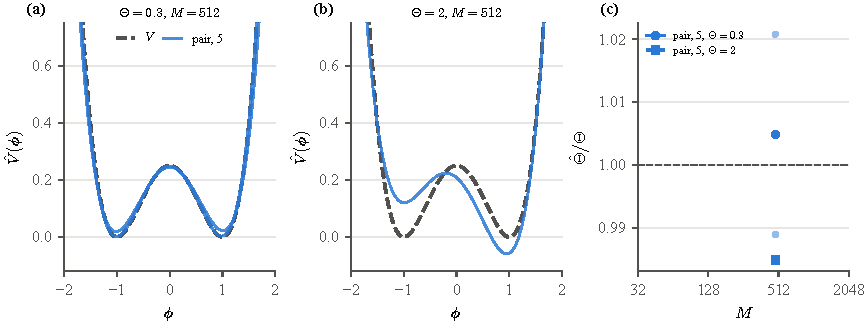
\includegraphics{fig-field-potential.pdf}
\caption{The physics read from kernels learned \emph{through the noise} (laptop preview, two seeds, not yet the
confirmatory run). (a) $\hat V$ from the five-parameter site energy at $\Th=0.3$, $M=512$ sequences, against the true
double well (dashed); a clean-data fit dotted. (b) The same at $\Th=2$, where the barrier is far below the
thermal energy and the data barely constrain it. (c) $\hat\Th/\Th$ against the number of sequences.}
\label{fig:potential}
\end{figure}

\subsection{What has been measured so far}

Table~\ref{tab:results} collects the numbers that matter for the paper, with their status. ``Frozen'' means the
output files are checksummed in the registry; ``preview'' means a laptop run on two cells and at most two seeds,
under the registered code but not the registered design. The confirmatory runs of E33 (sixteen seeds, six cells,
five kernel arms, two network architectures) are queued on the cluster.

\begin{table}[h]\centering\small
\caption{The main measurements on the $\phi^4$ laboratory. Score errors are pooled relative errors (\S\ref{sec:noise});
the base cell is $\Th=0.3$, $h=1$, $L=32$.}
\label{tab:results}
\begin{tabular}{@{}p{6.6cm}p{5.4cm}p{3.3cm}@{}}
\toprule
quantity & value & source, status \\
\midrule
Gaussian closure (linear floor), base cell & $0.269$ & E33 oracles, 16 seeds \\
floor along matched correlation, $\Th=0.3,0.5,1,2$ & $0.269,\ 0.114,\ 0.059,\ 0.041$ & E33 oracles \\
floor at fixed spacing $h=1$, $\Th=0.2\to2$ & $0.296\to0.184$, monotone & E32, frozen \\
Theorem~2 gap ratio at $t=3$ & $0.73$--$0.94$ & E32, frozen \\
mixture kernel through noise, base, $M=128$ and $512$ & $0.276,\ 0.272$ (no improvement with data) & preview \\
spline tilt through noise, base, $M=128$ and $512$ & $0.034,\ 0.039$ & preview \\
site energy through noise, base, $M=128$ and $512$ & $0.035,\ 0.021$ & preview \\
temperature read through noise, base, $M=512$ & $\hat\Th/\Th=1.005\pm0.023$, barrier $0.234$ & preview \\
clean fits, base, $M=2048$: site energy, spline, mixture & $0.005,\ 0.006,\ 0.27$ & preview \\
samples from the learned site energy: kinks, domain length & within $5\,\%$ and $2\,\%$ of the truth & preview \\
coarse kinks across lattice spacings, across strides & within $11\,\%$, within $8\,\%$ & E34, E36 \\
\bottomrule
\end{tabular}
\end{table}

Read the table as one story. The linear floor (Kalman on the covariance twin, \S\ref{sec:kalman}) leaves a quarter
of the score unexplained on the base cell, because the field's structure is non-Gaussian and the Hermite
argument (\S\ref{sec:hermite}) says that structure lives in high orders. The paper's mixture kernel cannot reach it
however much data it sees, because its drift is linear (\S\ref{sec:synthesis}). Kernels of the right class reach
errors seven to thirteen times smaller from a few hundred noised sequences, and their parameters return the temperature and
the potential that generated the data.

\subsection{Open questions}

\begin{itemize}
\item Do the confirmatory runs (sixteen seeds, six cells) confirm the preview's ordering, and does the
  five-parameter site energy beat the 25-parameter spline at small samples, as registered (E33 P7)?
\item Does a window network's error grow under lattice refinement while the learned kernel's does not (E33 P5,
  the note's ``sharp prediction'')?
\item Which kernel families survive subsampling, where the kernel $K^s$ is no longer a tilted walk (E36 P3)?
\item Does the augmented state repair a global latent sign (E35), completing the note's misspecification figure?
\item Should the paper present the pair energy as the general symmetric $W(a,a')$ or as the gradient form
  \eqref{eq:pairenergy}? The second is the whole class of discretised gradient SPDEs; the first would also cover
  couplings that are not of gradient type.
\end{itemize}

\paragraph{Check yourself.}
\begin{enumerate}[label=\thesection.\arabic*,leftmargin=2.2em]
\item For the Gaussian AR(1) chain at $\rho=0.85$ with $q=1-\rho^2$, what are the step variance $\gamma$ and the tilt
  $\log g$ of Proposition~\ref{prop:embed}?
\item A kernel fitted at the base cell ($h=1$, $s=0.8207$) has $\hat\gamma=0.450$. What temperature does it report?
\end{enumerate}

\appendix
\section{Notation}

\begin{center}\small
\begin{tabular}{@{}lp{4.6cm}@{\quad}lp{4.6cm}@{}}
\toprule
$a_i$ & clean standardised value at site $i$ & $x_i$ & noised observation \\
$t$, $\alpha=e^{-t}$, $\Delta=1-e^{-2t}$ & noise level and channel & $s_t(x)$ & data score $\nabla_x\log p_t$ \\
$K(a'\mid a)$ & transition kernel & $\pi$ & stationary density \\
$\fwd_i,\bwd_i$ & forward, backward messages & $\xi_i,\ \Xi$ & pair marginals, expected transition counts \\
$\ell_i(a)$ & likelihood $\N(x_i;\alpha a,\Delta)$ & $N_g$, $u_k$, $w_k$ & grid size, points, weights \\
$\rho$ & AR(1) coefficient & $\xi$ & correlation length in sites \\
$H_n$ & Hermite polynomial & $c_n$, $\kappa_n$ & Hermite coefficients, cumulants \\
$Q(\theta\mid\theta')$ & EM objective & $F(q,\theta)$ & evidence lower bound \\
$U_\theta$, $I(\theta)$ & parameter score, Fisher information & $\KL$ & Kullback--Leibler divergence \\
$\phi_i$, $h$, $\Th$ & field value, spacing, temperature & $V$ & double-well potential \\
$\En_h$ & lattice energy & $\mathsf T$, $\lambda_n$, $\psi_n$ & transfer operator and its eigenpairs \\
$g$, $Z_g$, $\gamma$ & tilt, normaliser, step variance & $f$, $W$ & site energy, pair energy \\
\bottomrule
\end{tabular}
\end{center}

\section{Where each idea lives in the code}

\begin{center}\small
\begin{tabular}{@{}p{6.0cm}p{9.6cm}@{}}
\toprule
idea & file \\
\midrule
grid BP, evidence, posterior means & \code{src/markov\_score/bp\_grid.py} \\
E-step (pair marginals), EM loop, Fisher's identity checks & \code{src/markov\_score/em.py}\newline \code{tests/test\_fisher\_bruteforce.py} \\
Gaussian closure = LMMSE (Prop.~1), the Kalman check & \code{tests/test\_gaussian\_bp\_equivalence.py}\newline \code{bp\_grid.grid\_bp\_projected\_batch} \\
mixture and neural kernels & \code{src/markov\_score/kernels.py} \\
$\phi^4$ transfer operator, $\psi_0$, exact sampling & \code{src/markov\_score/field.py} \\
tilted walk, closed-form $\pi_g$ and site energy & \code{src/markov\_score/tilted\_kernel.py} \\
pair energy with quartic site energy, readings of $\Th$ and $V$ & \code{src/markov\_score/pair\_energy\_kernel.py} \\
global sign latent and its repair by state augmentation & \code{src/markov\_score/augmented.py}\newline \code{experiments/e35\_state\_augmentation.py} \\
the experiments of this primer & \code{experiments/e32}\,--\,\code{e36}, registry in \code{experiments/registry/} \\
derivations in prose & \code{docs/FIELD\_MODEL.md}\newline \code{reports/field-laboratory-2026-10-01.pdf} \\
\bottomrule
\end{tabular}
\end{center}

\section{Answers to the check-yourself questions}

\begin{itemize}[leftmargin=2.6em,labelwidth=2.2em,align=left,itemsep=0.25em]
\item[\textbf{1.1}] $(x+h)^3-2x^3+(x-h)^3=6xh^2$, so the ratio is $6x=f''(x)$. The error in \eqref{eq:seconddiff} comes from the fourth
  derivative, which is zero for a cubic.
\item[\textbf{1.2}] Eigenvalue $3$ with eigenvector $(1,1)/\sqrt2$, eigenvalue $1$ with $(1,-1)/\sqrt2$. Since $3^N\gg1^N$, $A^Nv$ turns towards
  $(1,1)$, the positive Perron vector, unless $v$ is exactly perpendicular to it.
\item[\textbf{2.1}] Precisions add: $1/P'=1+1=2$, so the posterior is $\N(x/2,\,1/2)$. The guess splits the difference between the
  prior mean $0$ and the observation.
\item[\textbf{2.2}] $\kappa_4(x)=e^{-4}\times(-1.35)\approx-0.025$: at $t=1$ the noised marginal is almost Gaussian.
\item[\textbf{3.1}] $0.85^{10}\approx0.197$.
\item[\textbf{3.2}] Integrate both sides of \eqref{eq:detbal} over $a$: $\int\pi(a)K(a'\mid a)\dd a=\pi(a')\int K(a\mid a')\dd a=\pi(a')$.
\item[\textbf{4.1}] $(a,x)$ is jointly Gaussian with $\Cov(a,x)=\alpha$ and $\Var x=1$, so $\E[a\mid x]=\alpha x$ and the score is
  $(\alpha^2x-x)/\Delta=-x$. Indeed $x\sim\N(0,1)$, whose score is $-x$.
\item[\textbf{4.2}] $e^{2t}-1=1$, so $t=\tfrac12\log2\approx0.35$.
\item[\textbf{5.1}] $k=\alpha/(\alpha^2+\Delta)=1/\sqrt2\approx0.71$ and $P=(1-k\alpha)=\tfrac12$: one measurement at this level halves the variance.
\item[\textbf{5.2}] For Gaussians the posterior variance does not depend on the observed values, and conditioning on more
  variables cannot increase the expected posterior variance (law of total variance). So it can only shrink.
\item[\textbf{6.1}] $401^{32}\approx10^{83}$ terms against about $32\times401^2\approx5\times10^6$ multiplications.
\item[\textbf{6.2}] $\bwd_2(\mathrm R)=0.8\times0.1\times1+0.2\times0.8\times1=0.24$ (no umbrella on day three has probability $0.1$ if rainy, $0.8$
  if sunny). Then $0.342\times0.24+0.034\times0.66=0.1045$.
\item[\textbf{7.1}] By independence $\E e^{-ik(a+\sqrt\Delta z)}=\E e^{-ika}\,\E e^{-ik\sqrt\Delta z}$, and the transform of $\N(0,\Delta)$ is $e^{-\Delta k^2/2}$.
\item[\textbf{7.2}] $-\tfrac4{h^2}\sin^2(\pi/2)=-4/h^2$, the largest damping the grid can express.
\item[\textbf{8.1}] $\E[(Z^3-3Z)Z]=\E Z^4-3\E Z^2=3-3=0$.
\item[\textbf{8.2}] The part proportional to $e^{-4t}$ shrinks by $e^{-2}\approx0.14$; its squared error by $e^{-4}\approx0.018$.
\item[\textbf{9.1}] $Q$ is $\sum_k\sum_cr_{kc}[\log w_c+\log\N(y_k;\mu_c,\sigma_c^2)]$, a responsibility-weighted Gaussian log-likelihood for each
  component; maximising a weighted Gaussian likelihood gives weighted means and variances, and maximising
  $\sum r_{kc}\log w_c$ under $\sum_cw_c=1$ gives average responsibilities.
\item[\textbf{9.2}] The chain of inequalities in the monotonicity proof breaks at the middle step, so the evidence can
  decrease. Our kernels refuse such steps.
\item[\textbf{10.1}] $U=\sum_k(y_k-\mu)$ has variance $n$, so $I=1$ per draw and the bound is $1/n$; the sample mean has exactly this
  variance.
\item[\textbf{10.2}] Its expected value depends on the true law only through the covariance; two laws with the same
  covariance and different kurtosis give the same objective, so nothing in it can distinguish them.
\item[\textbf{11.1}] $\phi'=(1-\phi^2)/\sqrt2$, so $\phi''=-\sqrt2\,\phi\,\phi'=-\phi(1-\phi^2)=\phi^3-\phi$.
\item[\textbf{11.2}] $\pi\propto e^{-x^2/2\Th}$: the Gaussian $\N(0,\Th)$.
\item[\textbf{12.1}] $\int\mathsf T(\phi,\phi')\psi_0(\phi')\dd\phi'=\lambda_0\psi_0(\phi)$ by the eigen-equation, which cancels the denominator.
\item[\textbf{12.2}] $0.85^r<0.1$ for $r>\log0.1/\log0.85\approx14.2$, so after $15$ sites.
\item[\textbf{13.1}] $\gamma=q/\rho=0.2775/0.85\approx0.326$ and $\log g(a')=-(1-\rho)a'^2/2q\approx-0.270\,a'^2$.
\item[\textbf{13.2}] $\hat\Th=\hat\gamma s^2/h=0.450\times0.6736\approx0.303$, against the true $0.3$.
\end{itemize}

\section{Where to read more}
\sloppy

\begin{itemize}\small
\item Probability, Gaussians, EM, graphical models: C.~M.~Bishop, \emph{Pattern Recognition and Machine Learning} (2006),
  chapters 2, 8, 9 and 13.
\item Kalman filtering and smoothing: R.~E.~Kalman (1960), ``A new approach to linear filtering and prediction problems'';
  H.~E.~Rauch, F.~Tung and C.~T.~Striebel (1965), ``Maximum likelihood estimates of linear dynamic systems''.
\item Hidden Markov models: L.~R.~Rabiner (1989), ``A tutorial on hidden Markov models and selected applications in speech
  recognition''.
\item Belief propagation and factor graphs: J.~Pearl, \emph{Probabilistic Reasoning in Intelligent Systems} (1988);
  F.~R.~Kschischang, B.~J.~Frey and H.-A.~Loeliger (2001), ``Factor graphs and the sum-product algorithm''.
\item Markov random fields: J.~Besag (1974), ``Spatial interaction and the statistical analysis of lattice systems'';
  S.~Geman and D.~Geman (1984), ``Stochastic relaxation, Gibbs distributions, and the Bayesian restoration of images'';
  J.~Besag (1986), ``On the statistical analysis of dirty pictures''.
\item EM and its generalisations: A.~P.~Dempster, N.~M.~Laird and D.~B.~Rubin (1977), ``Maximum likelihood from incomplete
  data via the EM algorithm''; X.-L.~Meng and D.~B.~Rubin (1993), ``Maximum likelihood estimation via the ECM algorithm'';
  R.~M.~Neal and G.~E.~Hinton (1998), ``A view of the EM algorithm that justifies incremental, sparse, and other variants'';
  T.~A.~Louis (1982), ``Finding the observed information matrix when using the EM algorithm''.
\item Fisher information and quasi-likelihood: E.~L.~Lehmann and G.~Casella, \emph{Theory of Point Estimation};
  R.~W.~M.~Wedderburn (1974), ``Quasi-likelihood functions, generalized linear models, and the Gauss--Newton method'';
  H.~White (1982), ``Maximum likelihood estimation of misspecified models''.
\item Scores and diffusion models: B.~Efron (2011), ``Tweedie's formula and selection bias''; A.~Hyv\"arinen (2005),
  ``Estimation of non-normalized statistical models by score matching''; Y.~Song et al.\ (2021), ``Score-based generative
  modeling through stochastic differential equations''.
\item Langevin and Fokker--Planck: C.~W.~Gardiner, \emph{Handbook of Stochastic Methods}.
\item Allen--Cahn and the $\phi^4$ chain: S.~M.~Allen and J.~W.~Cahn (1979), ``A microscopic theory for antiphase boundary
  motion and its application to antiphase domain coarsening''; D.~J.~Scalapino, M.~Sears and R.~A.~Ferrell (1972),
  ``Statistical mechanics of one-dimensional Ginzburg--Landau fields''; J.~A.~Krumhansl and J.~R.~Schrieffer (1975),
  ``Dynamics and statistical mechanics of a one-dimensional model Hamiltonian for structural phase transitions'';
  M.~Kardar, \emph{Statistical Physics of Fields} (2007), for transfer matrices.
\item SPDEs, for later: G.~Da~Prato and J.~Zabczyk, \emph{Stochastic Equations in Infinite Dimensions}.
\end{itemize}


\end{document}
